\documentclass[12pt,a4paper]{article}
\usepackage[utf8]{inputenc}

\usepackage[top=2.5cm, bottom=2.5cm, left=3.5cm, right=2.5cm]{geometry}
\headsep 50pt

\usepackage{amsmath}
\usepackage{amsfonts}
\usepackage{amssymb}
\usepackage{graphicx}
\usepackage{float}
\usepackage[hyphens]{url}
\usepackage{hyperref}
\usepackage{gensymb}

% styling for VHDL
\usepackage{minted}

% Vertical spacing between \split environments
\setlength{\jot}{10pt}

% Todo command definition
\usepackage[bordercolor=white,backgroundcolor=gray!30,linecolor=black,colorinlistoftodos]{todonotes}
\newcommand{\rework}[1]{\todo[color=yellow,inline]{Rework: #1}}

% Colors
\usepackage{xcolor,colortbl}
\definecolor{program_color}{rgb}{0.83,0.47,0.13}
\definecolor{comment}{rgb}{0,0.41,0.16}

% Code styling
\usepackage{listings}
\lstdefinestyle{c}{
    language=C, 
    basicstyle=\scriptsize, 
    frame=single,
    keywordstyle=\color{program_color},
    numbers=left,
    tabsize=2,
    breaklines=true,
    captionpos=b,
    commentstyle=\color{comment}\ttfamily,
}

% Page footer
\usepackage{fancyhdr}
\usepackage{lastpage}
\usepackage[bottom]{footmisc}
\fancyfoot[C]{Page \thepage\ of \pageref{LastPage}}
\pagestyle{fancy}

% Huge page
\usepackage{pdfpages}
\newenvironment{hugepage}%
 {\clearpage
  %\changepage{297mm}{420mm}{25mm}{25mm}{5mm}{}{}{}{}} % switch to A3
  \changepage{}{210mm}{}{}{}{}{}{}{}}
 {\addtocounter{page}{-0} % decrement "page" counter variable by 1
  \clearpage
  \changepage{160mm}{247mm}{25mm}{25mm}{}{}{}{}{}} % back to A4
\usepackage{afterpage}
\usepackage{changepage}



% Import 'subsubsubsection' as 'paragraph'
\usepackage{titlesec}
\setcounter{secnumdepth}{4}
\titleformat{\paragraph}
{\normalfont\normalsize\bfseries}{\theparagraph}{1em}{}
\titlespacing*{\paragraph}
{0pt}{3.25ex plus 1ex minus .2ex}{1.5ex plus .2ex}


% \usepackage[utf8]{inputenc} % Required for inputting international characters
% \usepackage[T1]{fontenc} % Output font encoding for international characters

% \usepackage{mathpazo} % Palatino font

\setlength{\parindent}{0em}
\title{Extraction of printed circuit board parasitics of a switching power pole}
\author{University of Southern Denmark
 \\ \\ Students: \\ Imran Kamal, 210386 \\ David Kis-Toth, 060193\\  \\
Supervisors: \\ 
Morten Nymand: \href{mailto:mny@mci.sdu.dk}{\textit{mny@mci.sdu.dk}} \\
Christian Østergaard: \href{mailto:choe@mci.sdu.dk}{\textit{choe@mci.sdu.dk}} \\
Rakesh Ramachandran: \href{mailto:rar@mci.sdu.dk}{\textit{rar@mci.sdu.dk}} \\
Jesper Nielsen: \href{mailto:jesn@mci.sdu.dk }{\textit{jesn@mci.sdu.dk }}}
\date{Period: \\ 
 September 2019 - December 2019 (E19)}




\begin{document}

\begin{titlepage}
\thispagestyle{empty}
    \begin{figure}
        \vspace{-30pt}
        \centering
        
\includegraphics[width=0.4\textwidth]{pictures/general/SDU.png}
        \vspace{-50pt}
    \end{figure}
    \vspace{-1cm}

\end{titlepage}



\maketitle
\thispagestyle{empty}
    \begin{figure}
        \vspace{-25cm}
        \centering
        %\hspace{-1.5\textwidth}
        \colorbox{white}{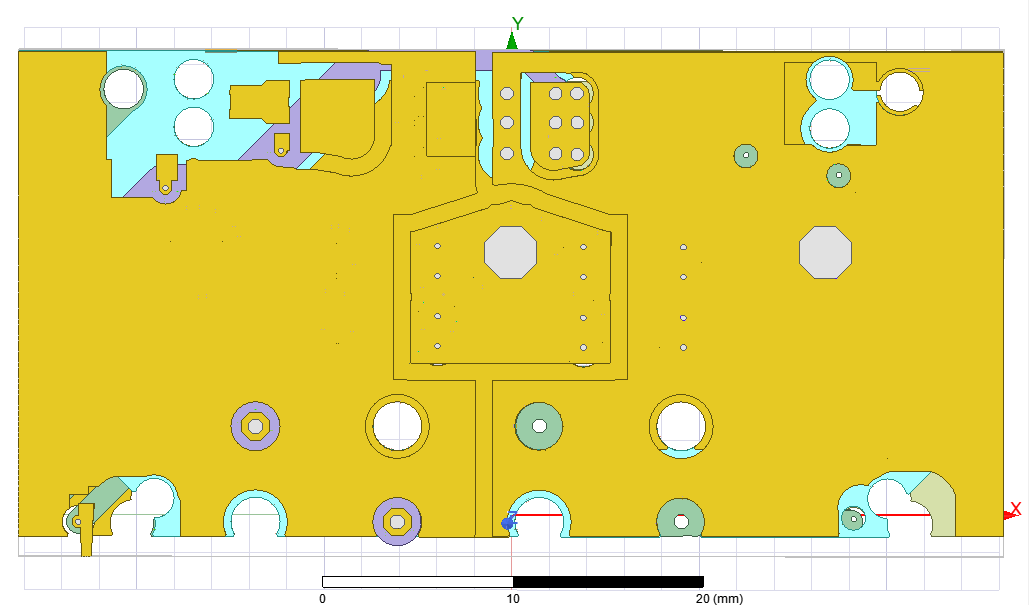
\includegraphics[width=1\textwidth,height=10cm]{pictures/general/PCB_mainpage.png}}
         \vspace{2cm}
    \end{figure}

% Front page
% 

\begin{titlepage} % Suppresses displaying the page number on the title page and the subsequent page counts as page 1
	\newcommand{\HRule}{\rule{\linewidth}{0.5mm}} % Defines a new command for horizontal lines, change thickness here
	
	\center % Centre everything on the page
	
	%------------------------------------------------
	%	Headings
	%------------------------------------------------
	
	\textsc{\LARGE Syddansk Universitet - Odense}\\[1.5cm] % Main heading such as the name of your university/college
	
	\textsc{\Large Masters in electronics - Second semester project}\\[0.5cm] % Major heading such as course name
	
	\textsc{\large Extraction of printed circuit board parasitics of a switching power pole}\\[0.5cm] % Minor heading such as course title
	
	%------------------------------------------------
	%	Title
	%------------------------------------------------
	
	\HRule\\[0.4cm]
	
	{\huge\bfseries Extraction of printed circuit board parasitics of a switching power pole}\\[0.4cm] % Title of your document
	
	\HRule\\[1.5cm]
	
	%------------------------------------------------
	%	Author(s)
	%------------------------------------------------
	
	\begin{minipage}{0.4\textwidth}
		\begin{flushleft}
			\large
			\textit{Authors}\\
			I. \textsc{Kamal}\\
			D. \textsc{Kis-Tóth}\\
		\end{flushleft}
	\end{minipage}
	~
	\begin{minipage}{0.4\textwidth}
		\begin{flushright}
			\large
			\textit{Supervisor}\\
			Morten \textsc{Nymand}\\
			Christian \textsc{Østergaard}\\
			Rakesh \textsc{Ramachandran}\\
			Jesper \textsc{Nielsen}
		\end{flushright}
	\end{minipage}
	
	% If you don't want a supervisor, uncomment the two lines below and comment the code above
	%{\large\textit{Author}}\\
	%John \textsc{Smith} % Your name
	
	%------------------------------------------------
	%	Date
	%------------------------------------------------
	
	\vfill\vfill\vfill % Position the date 3/4 down the remaining page
	
	{\large\today} % Date, change the \today to a set date if you want to be precise
	
	%------------------------------------------------
	%	Logo
	%------------------------------------------------
	
	%\vfill\vfill
	%\includegraphics[width=0.2\textwidth]{placeholder.jpg}\\[1cm] % Include a department/university logo - this will require the graphicx package
	 
	%----------------------------------------------------------------------------------------
	
	\vfill % Push the date up 1/4 of the remaining page
	
\end{titlepage}

\newpage
% Signatures
\section*{Signatures}


\begin{table}[H]
\begin{tabular}{lllll}
Approved:  & 
\includegraphics[width=0.25\textwidth, height=10mm]{pictures/general/Imran.PNG} &  & Approved:  & 
\includegraphics[width=0.25\textwidth, height=10mm]{pictures/general/david.PNG} \\ \cline{2-2} \cline{5-5} 
16-12-2019 & Imran Kamal&  & 16-12-2019 & David Kis-Toth \\
           &                          &  &            &                \\
     
\end{tabular}
\end{table}

% Abstract
\section{Abstract}

As the level of integration rises in electronic assemblies, difficulties with measuring the voltage and current waveforms emerge. It might be impossible to attach probes to the circuit without heavily modifying its behaviour. A possible solution for these problems is making finite element simulations of the circuit and its printed circuit board layout. \\

The project goes through the development of a SPICE model for one leg of a switch-mode power converter. The model should reflect the parasitic components inherent to the layout to demonstrate their effects on crucial voltage and current waveforms. Different iterations of the modelling process are described. Besides SPICE simulation, the parasitic extraction process is covered in detail.

% Preface
\section{Preface}
The project is the semester project on the 2nd semester of the Masters in Electronics course at The University of Southern Denmark and was done in the period from September 2019 to December 2019.


The group would like to thank our supervisors Morten Nymand, Christian Østergaard, Rakesh Ramachandran and Jesper Nielsen for the help and support throughout the project. 

\newpage
% Reading guide
\section{Reading guide}
The report is expected to be read in chronological order. \\

The reader is expected to have a knowledge of power electronics and circuit theory.

\medskip
The report has the following sections:

\medskip
\emph{Section \ref{sec:introduction} - Introduction} gives a short introduction to and outlines the goal of the project.

\medskip
\emph{Section \ref{sec:theory} - Theoretical background} investigates the mechanisms of oscillation and ringing, models for describing these phenomena and the importance of minimal circuit parasitics.

\medskip
\emph{Section \ref{sec:implementation} - Implementation} contains the modelling of the circuit under investigation in LTSpice, the different stages of modelling and usage of the ANSYS software suit.

\medskip
\emph{Section \ref{sec:discussion} - Discussion} goes through the interpretation of the results and possible further tasks.

\medskip
\emph{Section \ref{sec:conclusion} - Conclusion} outlines how the created model matches expectations.

\medskip
\emph{Section \ref{sec:abbreviation_list} - Abbreviation list} contains a list of all symbols together with a short description.


\medskip
\emph{Section \ref{sec:references} - References} contains a list of the sources used.


\newpage
\tableofcontents
\newpage
% Introduction
\section{Introduction}
\label{sec:introduction}

Miniaturization is a key goal in every field of electronic development. Higher efficiency and lower amount of material used for a given purpose go hand in hand. Improving these metrics means cheaper products in the long run. Since the size of magnetic components in a power converter is inversely proportional to the switching frequency, it is also beneficial to raise the switching frequency to the point where it is in equilibrium with the capacitive losses of the MOSFET. Other factors also apply for selecting the switching frequency but investigating them is out of the scope of this report. \\

With the level of integration increasing in printed circuit board assemblies (PCBAs), the effect of parasitic inductances, capacitances and resistances becomes more of a concern. In the case of switch mode power converters, the high-frequency gate signal of power MOSFETs is exceptionally susceptible to noise. For this reason, shielding the gate signal from other, quickly changing and/or high-amplitude signals is crucial. Providing the shortest possible return path for the driver current is also important. \\

One ever-present source of noise is the complementary switch element of a switching power pole. Creating a PCB layout with as small as possible parasitic inductances, capacitances and resistances is an even more crucial task. \\

It can be difficult to measure voltage and especially current waveforms in tightly-packed PCBAs. Installing testpoints introduces substantial parasitics. Touching the assemblies with a voltage probe introduces the parasitics of the measurement instrument. As these are comparable to those of a good layout, the engineer cannot be certain that they observe the behaviour of the original circuit or that of the superseding one. Modifying the circuit to accept a current probe is a characteristic modification as well. \\

The aforementioned reasons necessitate the use of finite element modeling techniques. Creating models of circuits that can be verified by measurement is the first step toward being able to consistently model super-miniature circuits. Extracting parasitics of a known, well-designed switching circuit and applying them to the SPICE model of this circuit is the scope of this project. Exploring modelling methods and the usage of associated software makes performing more complicated future modelling tasks possible. \\

\newpage
% Theoretical background
\section{Theoretical background}
\label{sec:theory}

The theoretical background of the project is described in this section. Section \ref{sec:oscillators} deals with oscillator models for power MOSFET topologies. Section \ref{sec:circumstances_for_osc} explains the circumstances that enable oscillation. Section \ref{sec:ringing} briefly introduces ringing.

% Oscillators
\subsection{Oscillators}
\label{sec:oscillators}

Circuit parasitics can lead to the degradation of the FET gate signals. One way to grasp this effect is to look at the parasitic feedback circuit that leads to ringing and oscillation of the switches. For the sake of simplicity, the case of a single MOSFET is examined throughout Section \ref{sec:oscillators}. \\

This section is mainly based on a Toshiba application note \cite{Toshiba_app_note}.

\subsubsection{Causes of oscillation}
\label{sec:causes_of_osc}

False switching happens when a ringing or oscillating gate signal repeatedly turns the MOSFET on and off. This could cause excess power losses and permanent damage of the FET.

The three major causes of oscillation and ringing are the following: \\

\begin{itemize}
    \item An oscillation circuit is formed of the parasitic components and the feedback gain of the FET.
    \item A drain-source surge voltage during turn-off could reach the gate via feedback through the gate-drain capacitance $C_{GD}$.
    \item If the turn-off di/dt induces high enough voltage in the source stray inductances, the gate-source loop could go into LCR resonance. Stray inductance is a major contributor to potential ringing.
\end{itemize}

\subsubsection{Oscillation networks}
\label{sec:osc_network}

Oscillation happens when a circuit experiences voltage and current vibration without excitation from an external vibration source. Since all real-world circuits have resistance, oscillations dampen over time unless energy is fed into the network. In order for oscillation to occur, the feedback signal must match the phase and frequency of the input signal and have high enough amplitude to compensate for losses.

\subsubsection{Feedback circuit}
\label{sec:feedback_circuit}

The circuit in Figure \ref{fig:feedback_cl} shows the basic feedback network where

\begin{itemize}
    \item $v_i = $ input voltage
    \item $v_o = $ output voltage
    \item $A = $ loop gain
    \item $H = $ feedback factor
    \item $v_1 = $ input voltage applied to the amplifier
    \item $v_2 = $ feedback voltage
    \item $G_O = $ open-loop gain
    \item $G_C = $ overall, closed-loop gain
\end{itemize}

\begin{figure}[H]
	\centering
	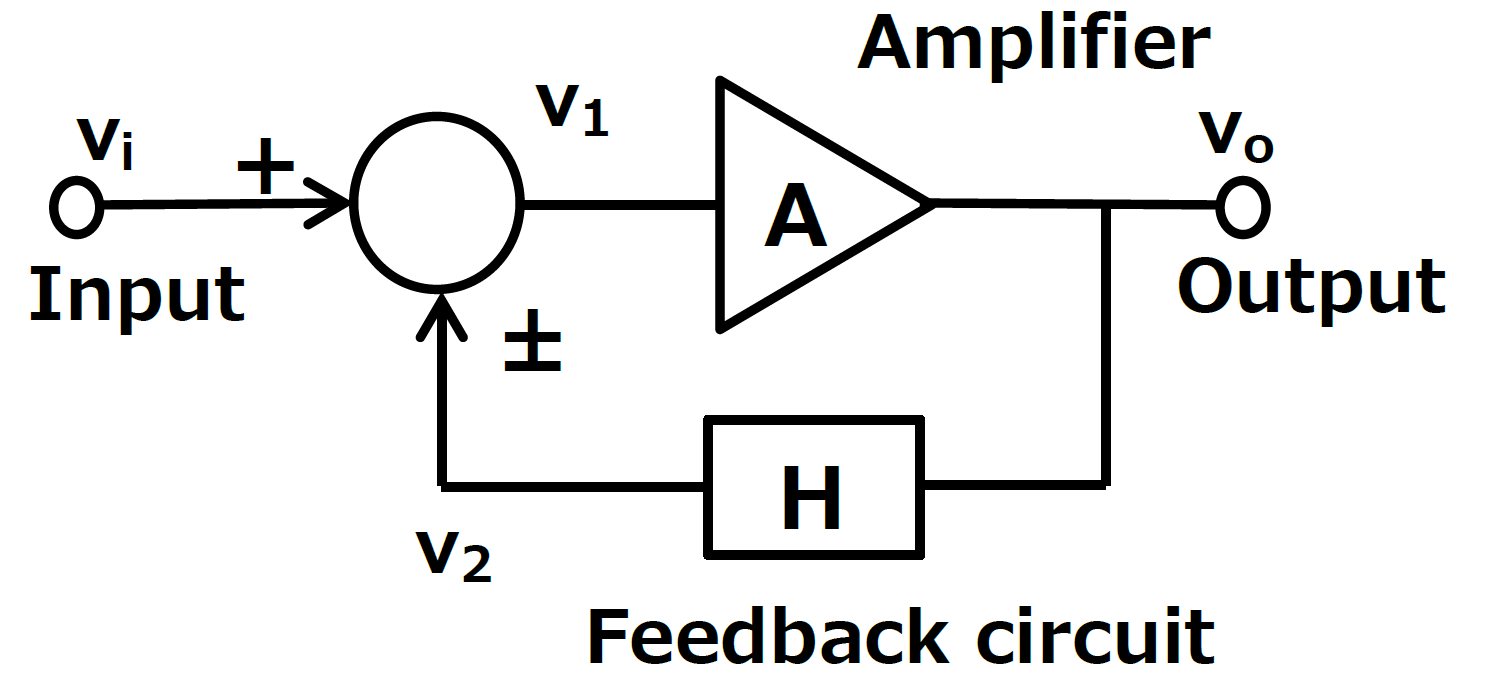
\includegraphics[width=0.4\textwidth]{pictures/theory/feedback_cl.png}
	\caption{Closed-loop feedback circuit}
	\label{fig:feedback_cl}
\end{figure}

To calculate the overall gain $G_C$, first, the open-loop transfer function should be specified:

\begin{equation}
    v_2 = AHv_1
\end{equation}

Dividing by $v_1$:

\begin{equation}
    G_O = \frac{v_2}{v1} = AH
\end{equation}

It can be seen that

\begin{equation}
    V_o = Av_1
\end{equation}

and

\begin{equation}
    V_1 = v_i + Hv_o
\end{equation}

combined yield

\begin{equation}
    v_o = A(v_i + Hv_o) = \frac{A}{1-AH}v_i
\end{equation}

From here, it is only one more step to get

\begin{equation}
    Gc = \frac{v_o}{v_i} = \frac{A}{1-AH}
    \label{eq:gc}
\end{equation}

\subsection{Circumstances for oscillation}
\label{sec:circumstances_for_osc}

If there is a positive feedback with $AH = 1$ from Equation \ref{eq:gc}; $G_c$ becomes infinite, prompting the network to oscillate. If we represent the $AH$ loop gain with a complex number of the form $a + jb$, oscillation occurs when $Re(AH) \geq 1$.

\subsubsection{MOSFET oscillation}
\label{sec:mosfet_osc}

If the parasitics are not keenly controlled, MOSFETs' high transconductance ($g_m$) and parasitic capacitances complemented by stray inductances make them susceptible to oscillation. $g_m$ is low when the MOSFET is in a steady state, so quick transient periods are of concern: when the load is shorted or switching occurs.

\subsubsection{MOSFET feedback loop}
\label{sec:mosfet_feedback_loop}

This section discusses the model for the single MOSFET feedback loop with ideal reactances seen in Figure \ref{fig:osc_model}. The resistance of the reactances is zero, current does not flow between the MOSFET and the reactances. Hence, Figure \ref{fig:osc_model2} is a good approximation.

\begin{figure}[H]
	\centering
	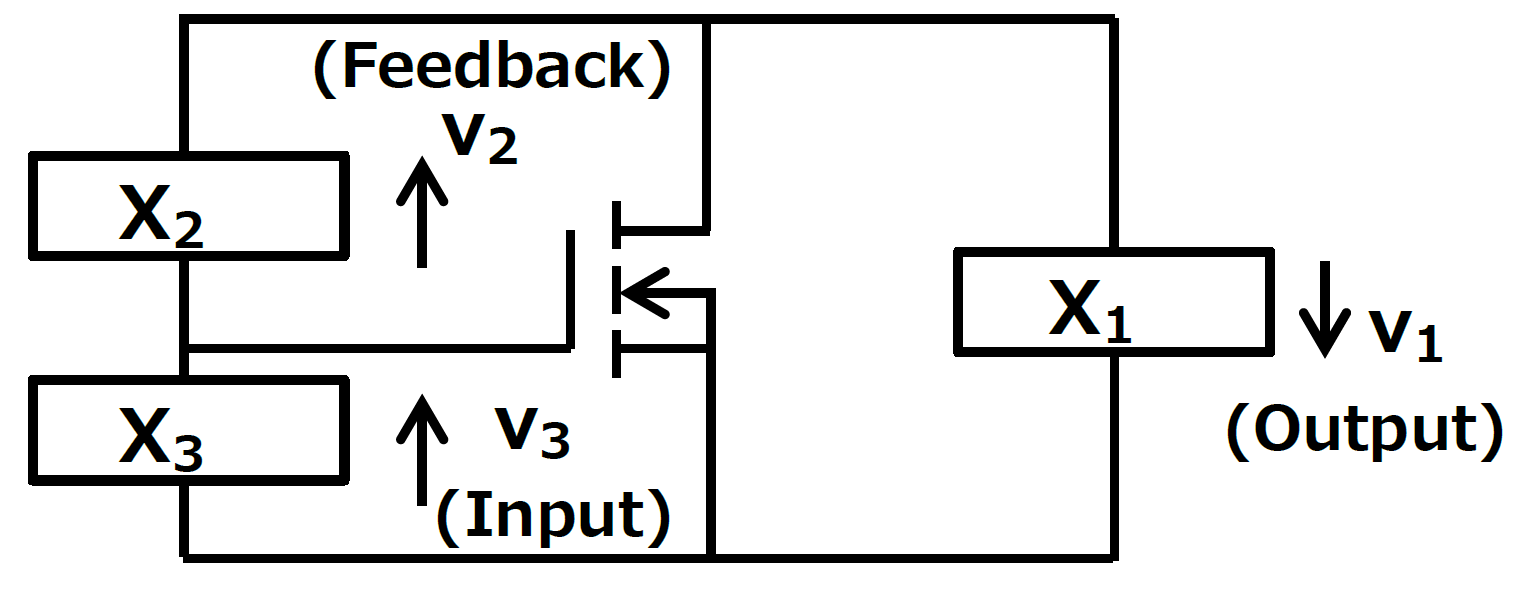
\includegraphics[width=0.4\textwidth]{pictures/theory/feedback_model.PNG}
	\caption{Circuit of an oscillation model}
	\label{fig:osc_model}
\end{figure}

\begin{figure}[H]
	\centering
	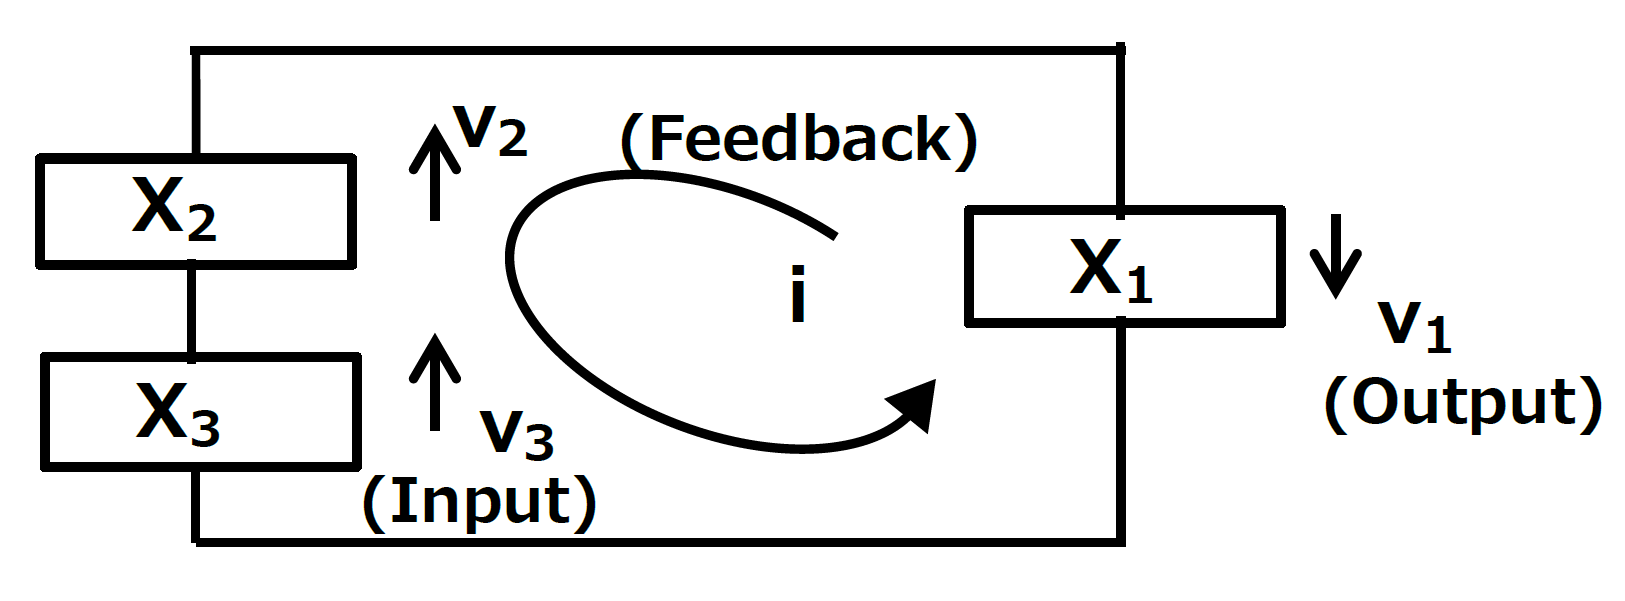
\includegraphics[width=0.4\textwidth]{pictures/theory/feedback_model_2.PNG}
	\caption{Current in the oscillation network}
	\label{fig:osc_model2}
\end{figure}

Kirchhoff's laws applied to Figure \ref{fig:osc_model2} yield

\begin{equation}
    v_1+v_2+v_3 = i(X_1+X_2+X_3) = 0
\end{equation}{}

and $i \neq 0 $ so

\begin{equation}
X_1+X2+X_3 = 0
\end{equation}

must be true. \\

The positive feedback loop can only occur when the input is in phase with the output. This happens when $X_1$ and $X_3$ are of the same property and $X_2$ is different. Circuits fulfilling the above requirements are Colpitts (Figure \ref{fig:colpitts_1}) and Hartley (Figure \ref{fig:hartley_1}) oscillators.

\begin{figure}[H]
	\centering
	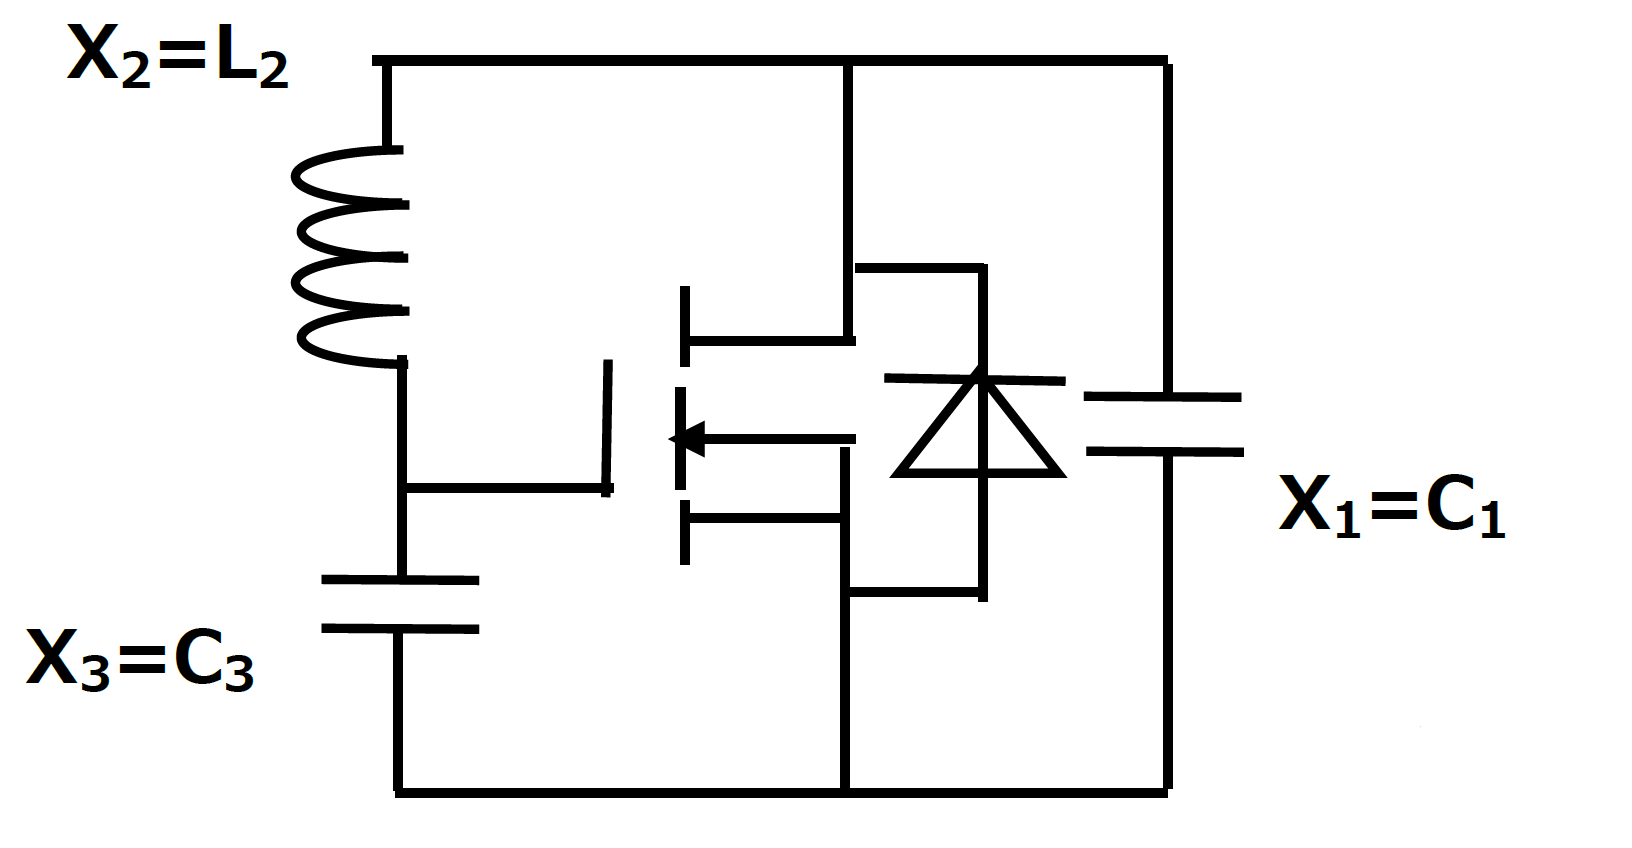
\includegraphics[width=0.4\textwidth]{pictures/theory/colpitts_1.PNG}
	\caption{Colpitts oscillator}
	\label{fig:colpitts_1}
\end{figure}

\begin{figure}[H]
	\centering
	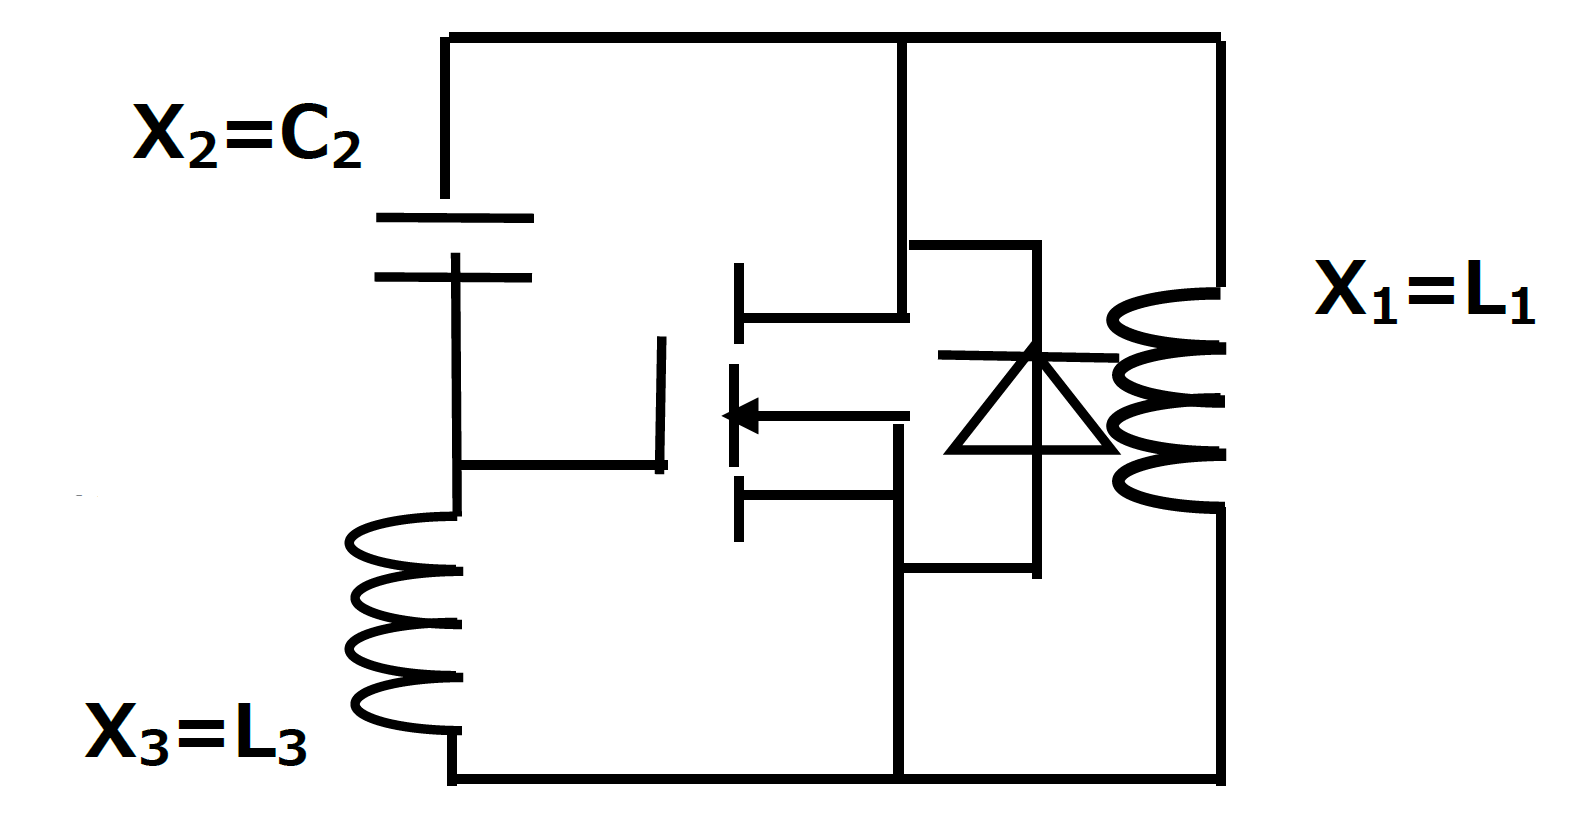
\includegraphics[width=0.4\textwidth]{pictures/theory/hartley_1.PNG}
	\caption{Hartley oscillator}
	\label{fig:hartley_1}
\end{figure}

\begin{figure}[H]
	\centering
	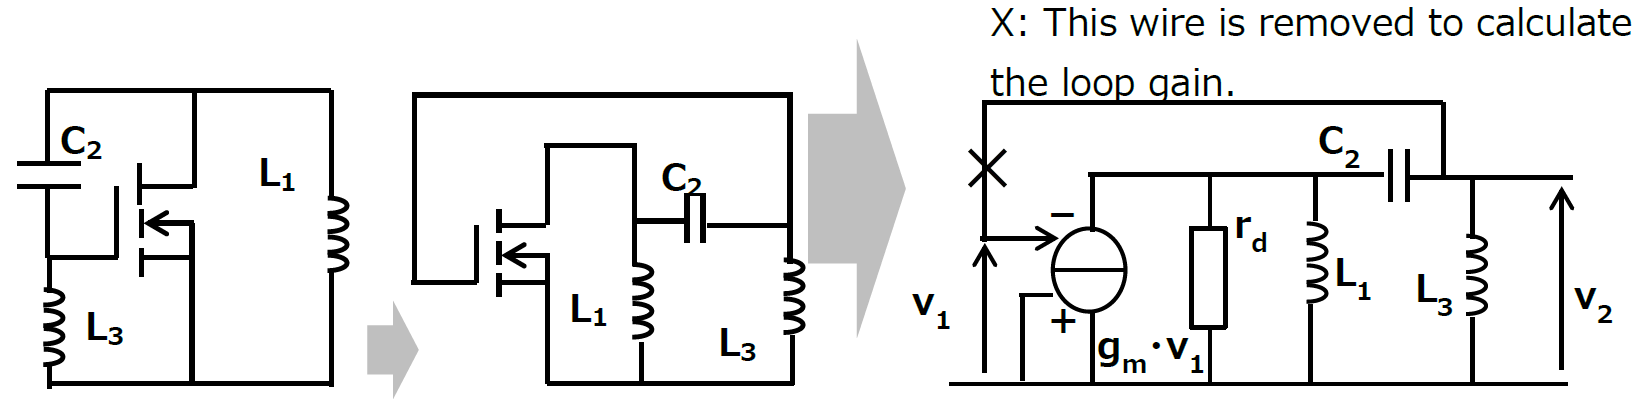
\includegraphics[width=\textwidth]{pictures/theory/hartley_2.PNG}
	\caption{Equivalent circuit of Hartley oscillator}
	\label{fig:hartley_2}
\end{figure}

Writing up the transfer function based on Figure \ref{fig:hartley_2} and performing further arithmetic actions yields the following:


\begin{equation}
    \omega = \frac{1}{\sqrt{(L_1 + L_3)C_2}}
    \label{eq:omega_hartley}
\end{equation}

\begin{equation}
    g_m \cdot r_D \geq \frac{L_1}{L_3}
    \label{eq:gain_hartley}
\end{equation}

Equation \ref{eq:omega_hartley} and \ref{eq:gain_hartley} gives the formula for calculating the oscillation frequency and the loop gain for a given set of parameters.

\subsection{Ringing}
\label{sec:ringing}

When switching off the MOSFET, drain di/dt and stray inductances can cause a $V_{DS}$ voltage surge that gets coupled to the gate. This ringing voltage can perturbate the gate signal so greatly that it repeatedly turns on and off, driving the MOSFET into oscillation. \\

The amplitude of the surge voltage depends on the value of the parasitic inductance and the changing rate of the drain current:

\begin{equation}
    V_{Surge} = L_{S2} \frac{di}{dt}
\end{equation}

\begin{figure}[H]
	\centering
	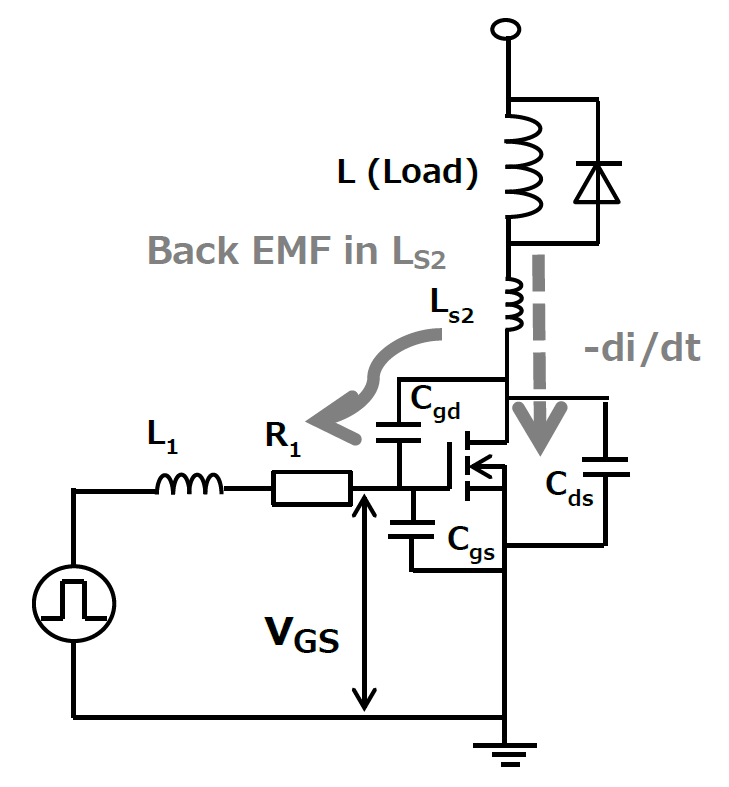
\includegraphics[width=0.4\textwidth]{pictures/theory/ringing_coupling.PNG}
	\caption{Ringing waveforms}
	\label{fig:ringing_coupling}
\end{figure}

The voltage gets coupled to the gate via $C_{gd}$, resulting in waveforms similar to those of in Figure \ref{fig:ringing_wf}

\begin{figure}[H]
	\centering
	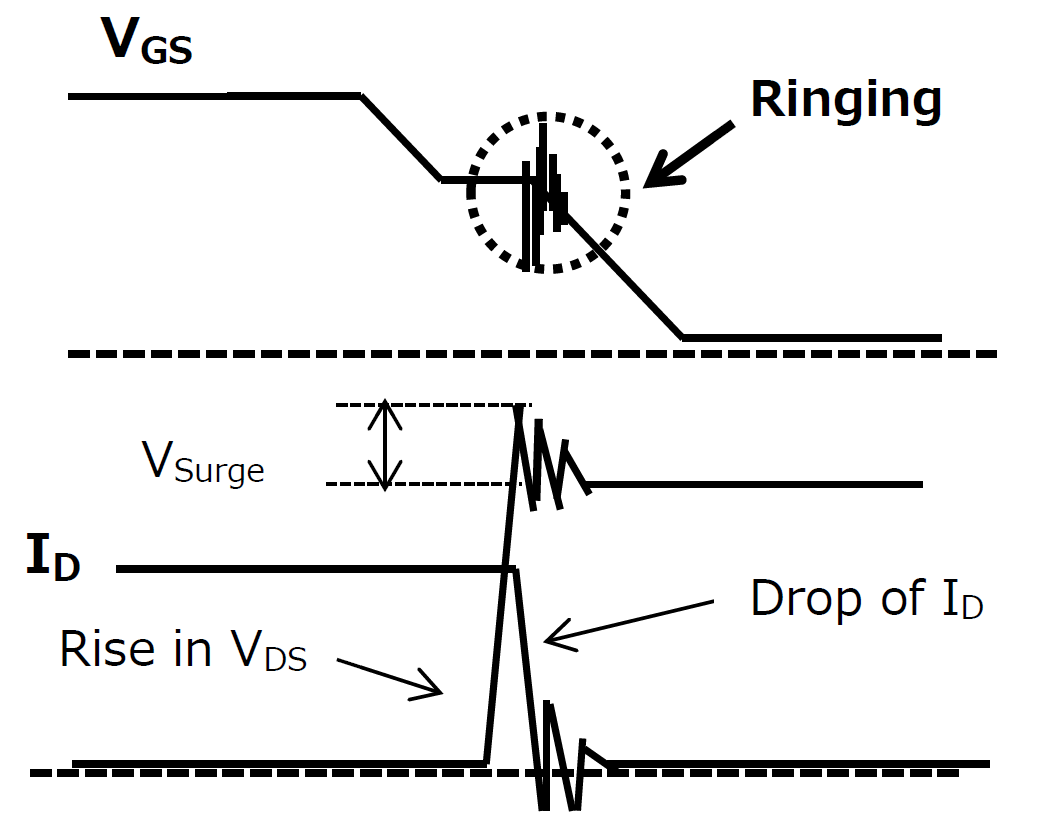
\includegraphics[width=0.4\textwidth]{pictures/theory/ringing_wf.PNG}
	\caption{Ringing waveforms}
	\label{fig:ringing_wf}
\end{figure}

High gate inductance and high driver turn-on currents associated with quick switching can also cause ringing. Dampening it by adding a resistor to the gate track brings additional losses. Furthermore slowing switching down increases the time slot when the MOSFET is subject to voltage and current at the same time, further increasing losses. Additional resistance may also prohibit operation at the desired frequency. Reducing parasitic inductances proves to be the desired action again.



\newpage
% Implementation
\section{Implementation}
\label{sec:implementation}

% Material requirements
\subsection{Material requirements}
\label{sec:material_requirements}

\subsubsection{Software}
\label{software_requirements}

Finding the right software suit proved somewhat difficult. ANSYS has several components that can cooperate and are integrated. The ones used were ANSYS Electronics Desktop and SIWave. Although the installer is not easily available, they all work with SDU's licence server. LTSpice is available for free. The Altium-files were provided as exported ODB++ and 3D PDF files, this way no Altium installation was required.

\subsubsection{Hardware}
\label{hardware_requirements}

Since this project is entirely about simulation, raw material costs are virtually null. Using a 3D mouse makes manipulating ANSYS incredibly easier but it is manageable without one. Individual simulation times with a mid-range laptop are tolerable.

% Overview
\subsection{Overview}
\label{sec:overview}

At the beginning of the project, we got the schematic and layout of a single leg of a switch-mode power converter. The plan was to build a working LTSpice model of this using the manufacturer model of the MOSFET. Since it is just one leg and no load is attached in the original layout, it was complemented with a load resistor in a half-bridge inverter fashion. This mode of operation has the least deviation from the original layout while it remains easy to control. \\

Gradually extracting parasitics from the layout and adding them to the Spice model as linear, lumped components was the method ofhttps://www.overleaf.com/project/5dea5a6aca434e00011844e4 work. The goal was to get the characteristic parasitics, see their effects one by one, then arrive to a plausibly complex model that could later be verified by measurements.

% Plain circuit
\subsection{Plain circuit}
\label{sec:plain}

Creating the LTSpice model of the plain circuit set the baseline for all further work. Interpreting Figure \ref{fig:schematic_altium_1} and \ref{fig:schematic_altium_2} yielded what can be seen in Figure \ref{fig:spice_plain_1}. The original converter has about $900V$ over the power pole, so a symmetric 450V supply was chosen.

\begin{figure}[H]
	\centering
	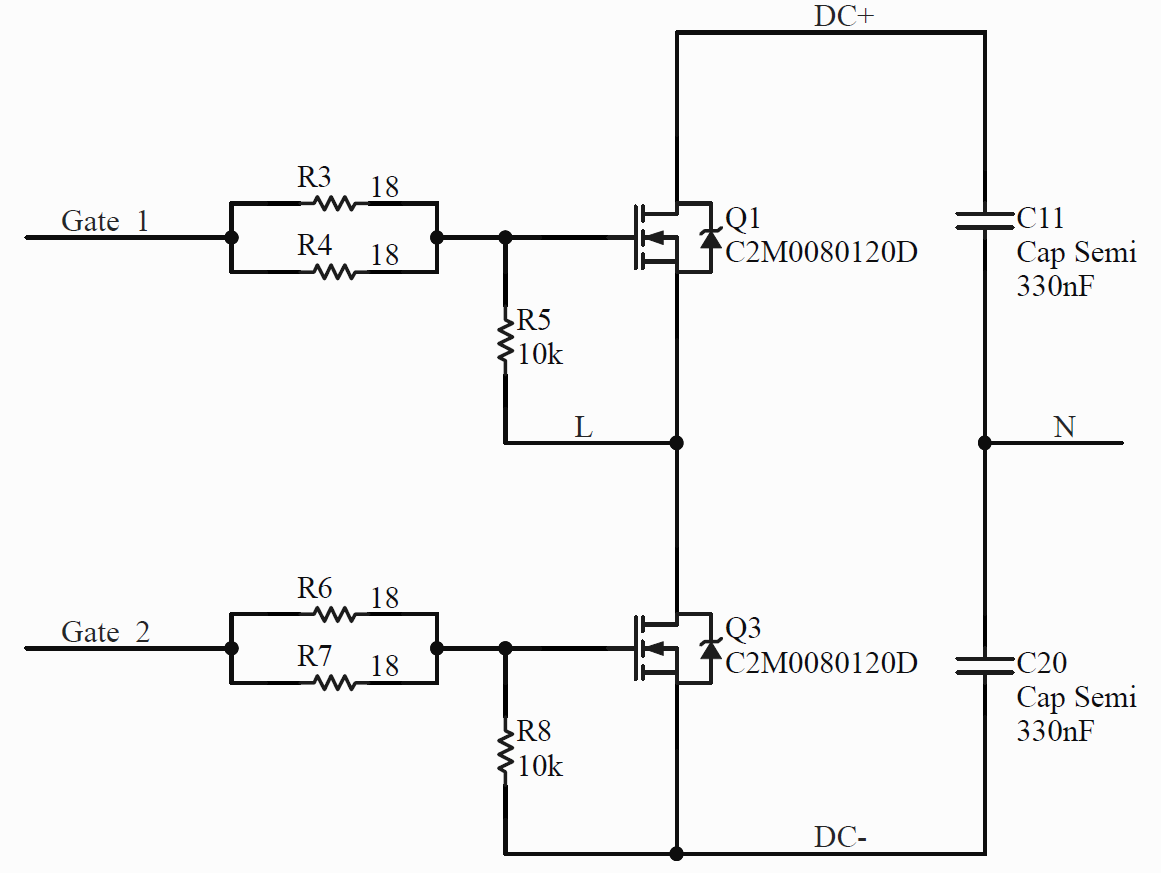
\includegraphics[width=\textwidth]{pictures/implementation/schematic_altium_1.PNG}
	\caption{Schematic of power pole}
	\label{fig:schematic_altium_1}
\end{figure}

\begin{figure}[H]
	\centering
	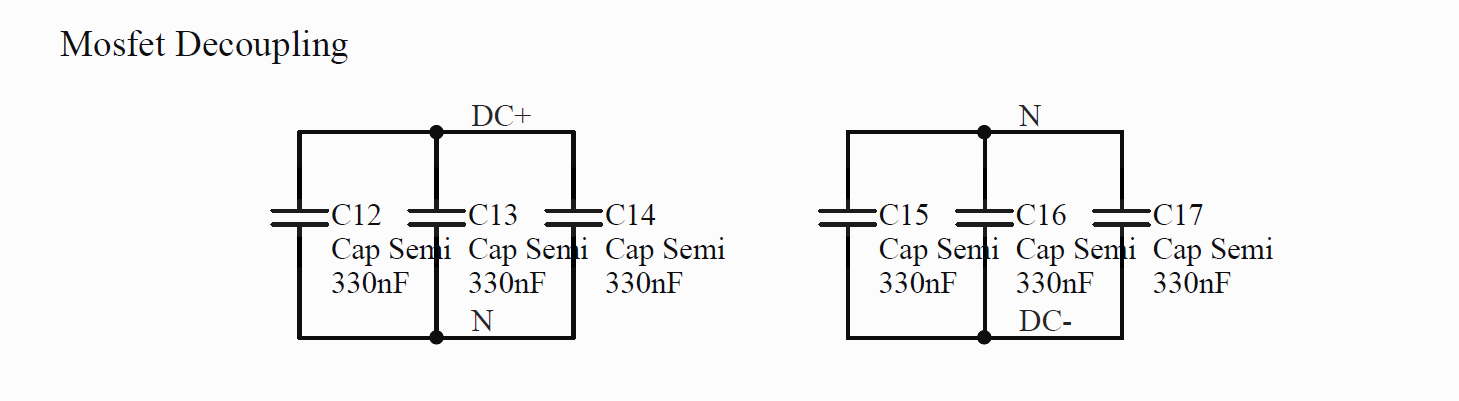
\includegraphics[width=\textwidth]{pictures/implementation/schematic_altium_2.PNG}
	\caption{Decoupling capacitors parallel to C11 and C20}
	\label{fig:schematic_altium_2}
\end{figure}

\begin{figure}[H]
	\centering
	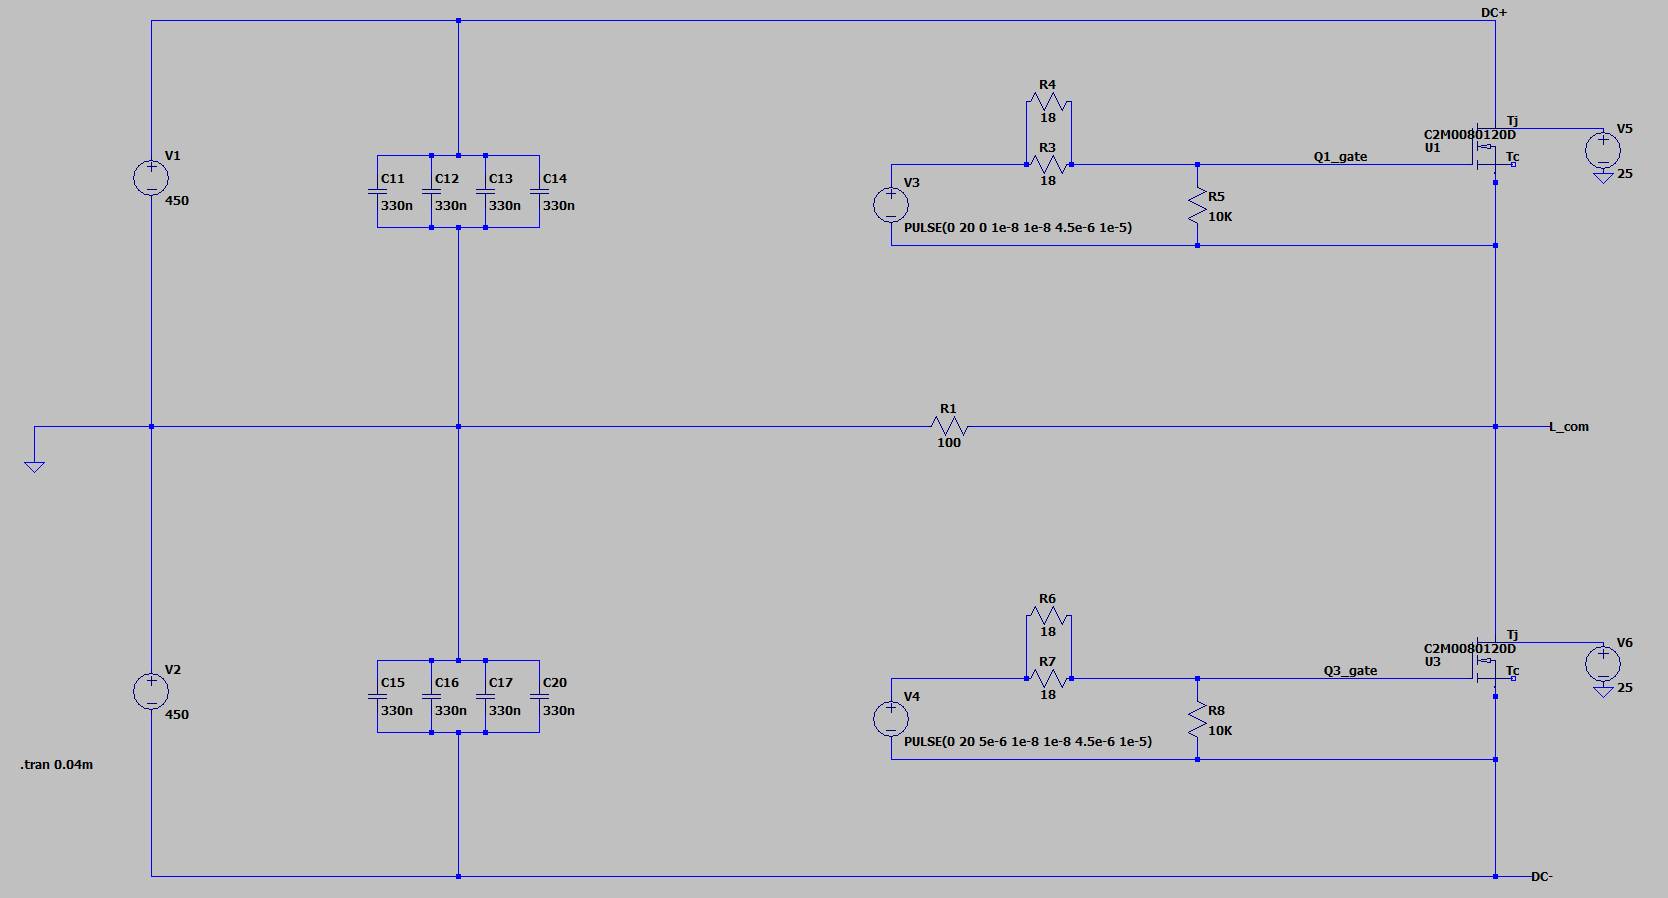
\includegraphics[width=\textwidth]{pictures/implementation/plain/spice_plain_1.PNG}
	\caption{LTSpice model of plain circuit}
	\label{fig:spice_plain_1}
\end{figure}

The only nonideality in this circuit is the manufacturer model \cite{mosfet_2} of the MOSFET Cree C2M0080120D. As most of the gate-source voltage dependent parameters were specified at $V_{GS} = 20V$ in its datasheet \cite{mosfet}, a $V_{GS} = 20V$ was chosen. The original converter runs at a switching frequency of $100 kHz$, so it was natural to pick that. On and off slopes should be quick enough to challenge the layout, so they were chosen to be 2 orders of magnitude quicker than the period time. 10\% deadtime was also included to prevent shoot-through at switching.\\

The MOSFET model supports thermal simulation that has not been utilized. The junction temperature $T_j$ was fixed at 25\textcelsius.

\subsubsection{Waveforms}
\label{sec:plain_waveforms}

The simulated waveforms look plausible. Some cross-coupling can be seen at the moment of the switching but this is not enough to trigger false turn on-off cycles.

Figure \ref{fig:plain_gates_1} shows two whole cycles as an overview, Figure \ref{fig:plain_gates_2} shows the transient where $ Q_1$ $V_{GS}$ turns off, Figure \ref{fig:plain_gates_3} depicts the other end of that cycle. Figure \ref{fig:plain_load} demonstrates the voltage and current of the load.

\begin{figure}[H]
	\centering
	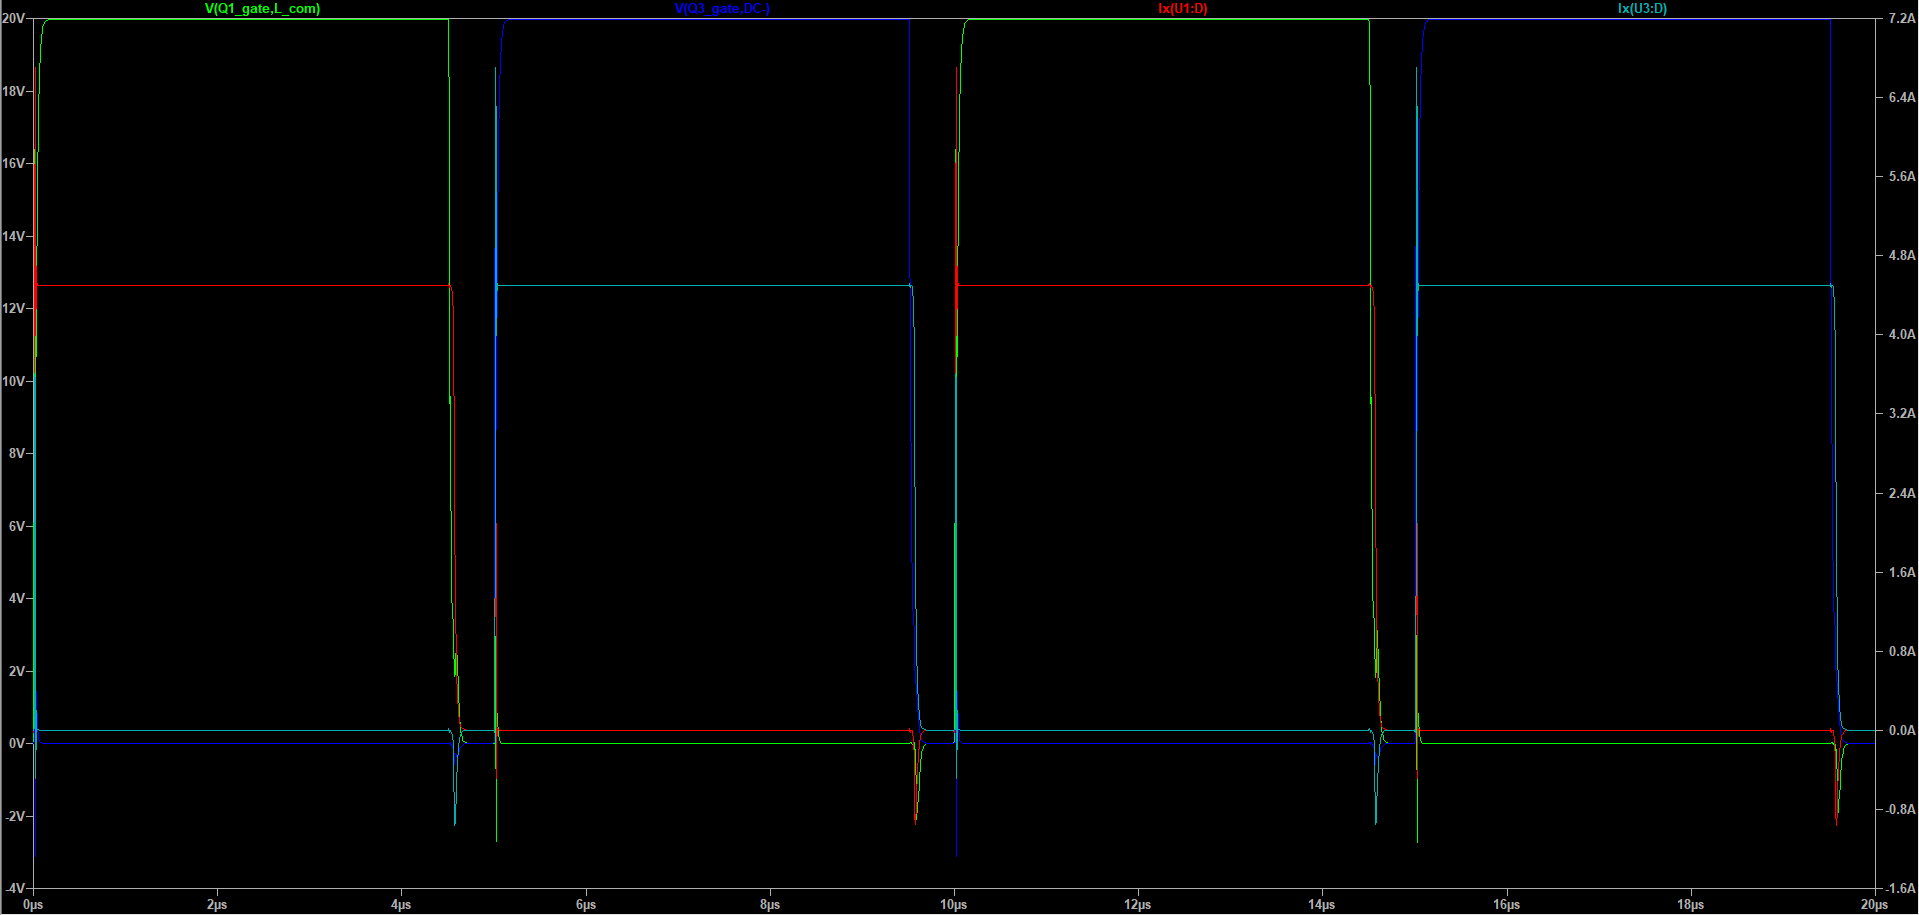
\includegraphics[width=\textwidth]{pictures/implementation/plain/plain_gates_1.PNG}
	\caption{Overview of the gate voltages and drain currents}
	\label{fig:plain_gates_1}
\end{figure}

\begin{figure}[H]
	\centering
	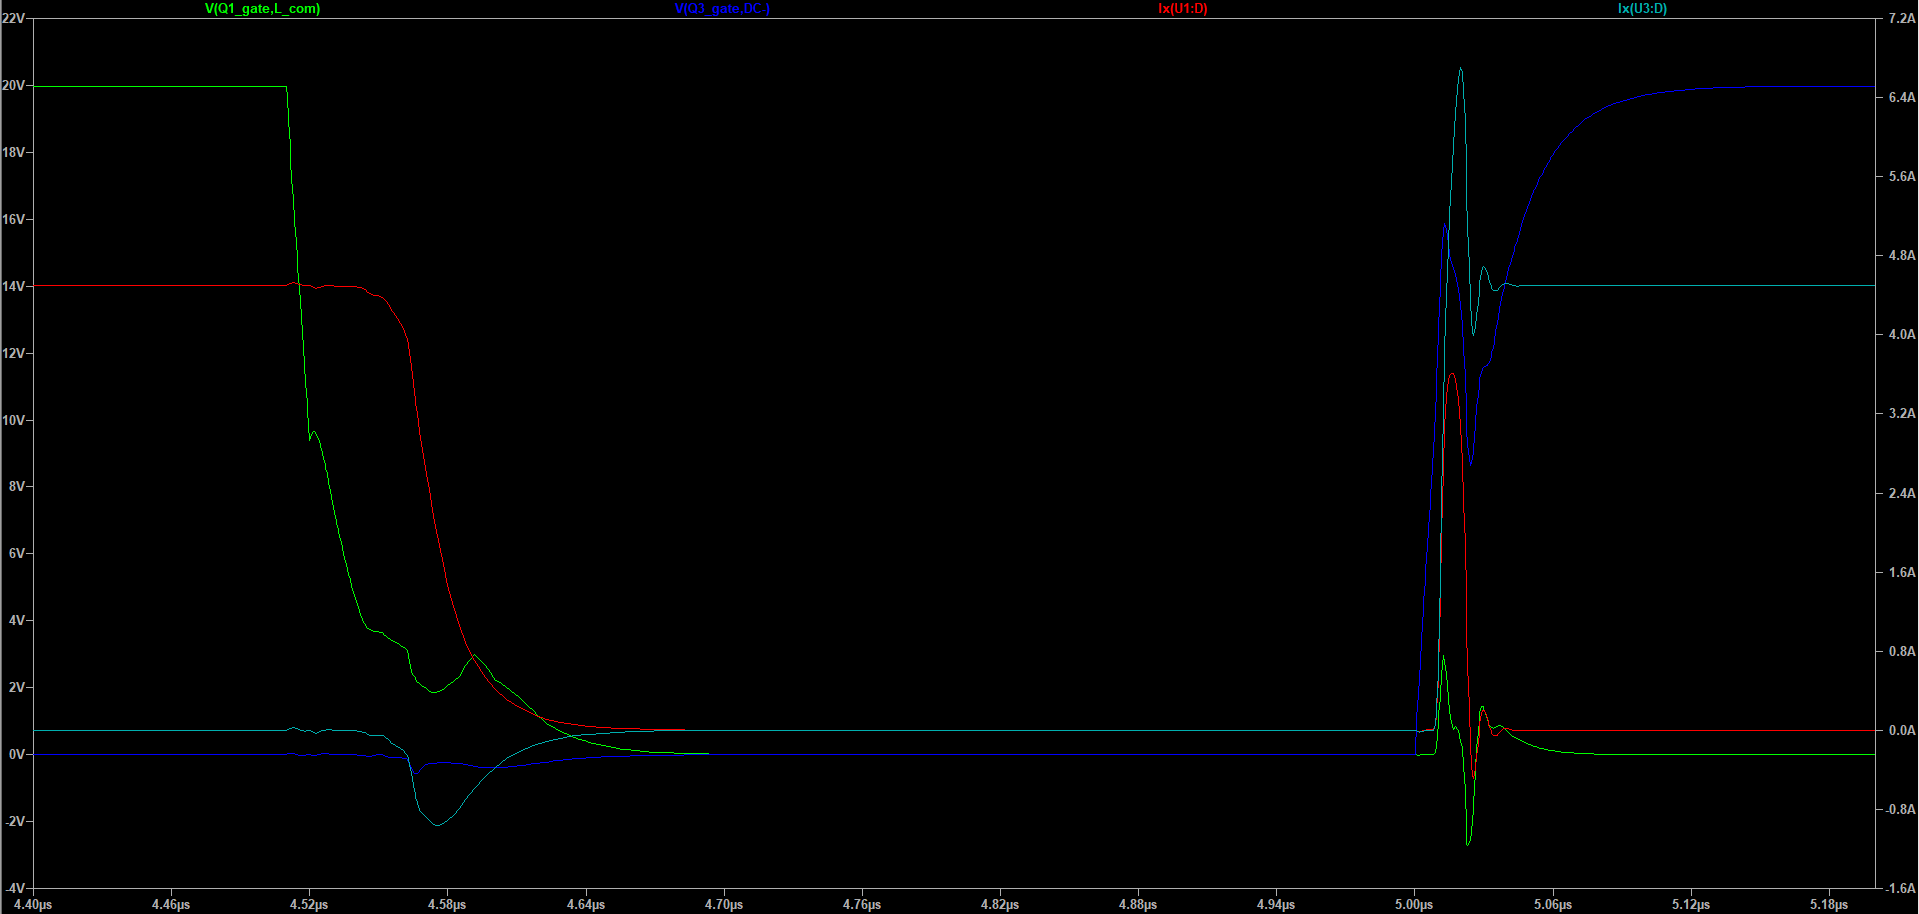
\includegraphics[width=\textwidth]{pictures/implementation/plain/plain_gates_2.PNG}
	\caption{Q1 turn off transient, gate voltages and drain currents}
	\label{fig:plain_gates_2}
\end{figure}

\begin{figure}[H]
	\centering
	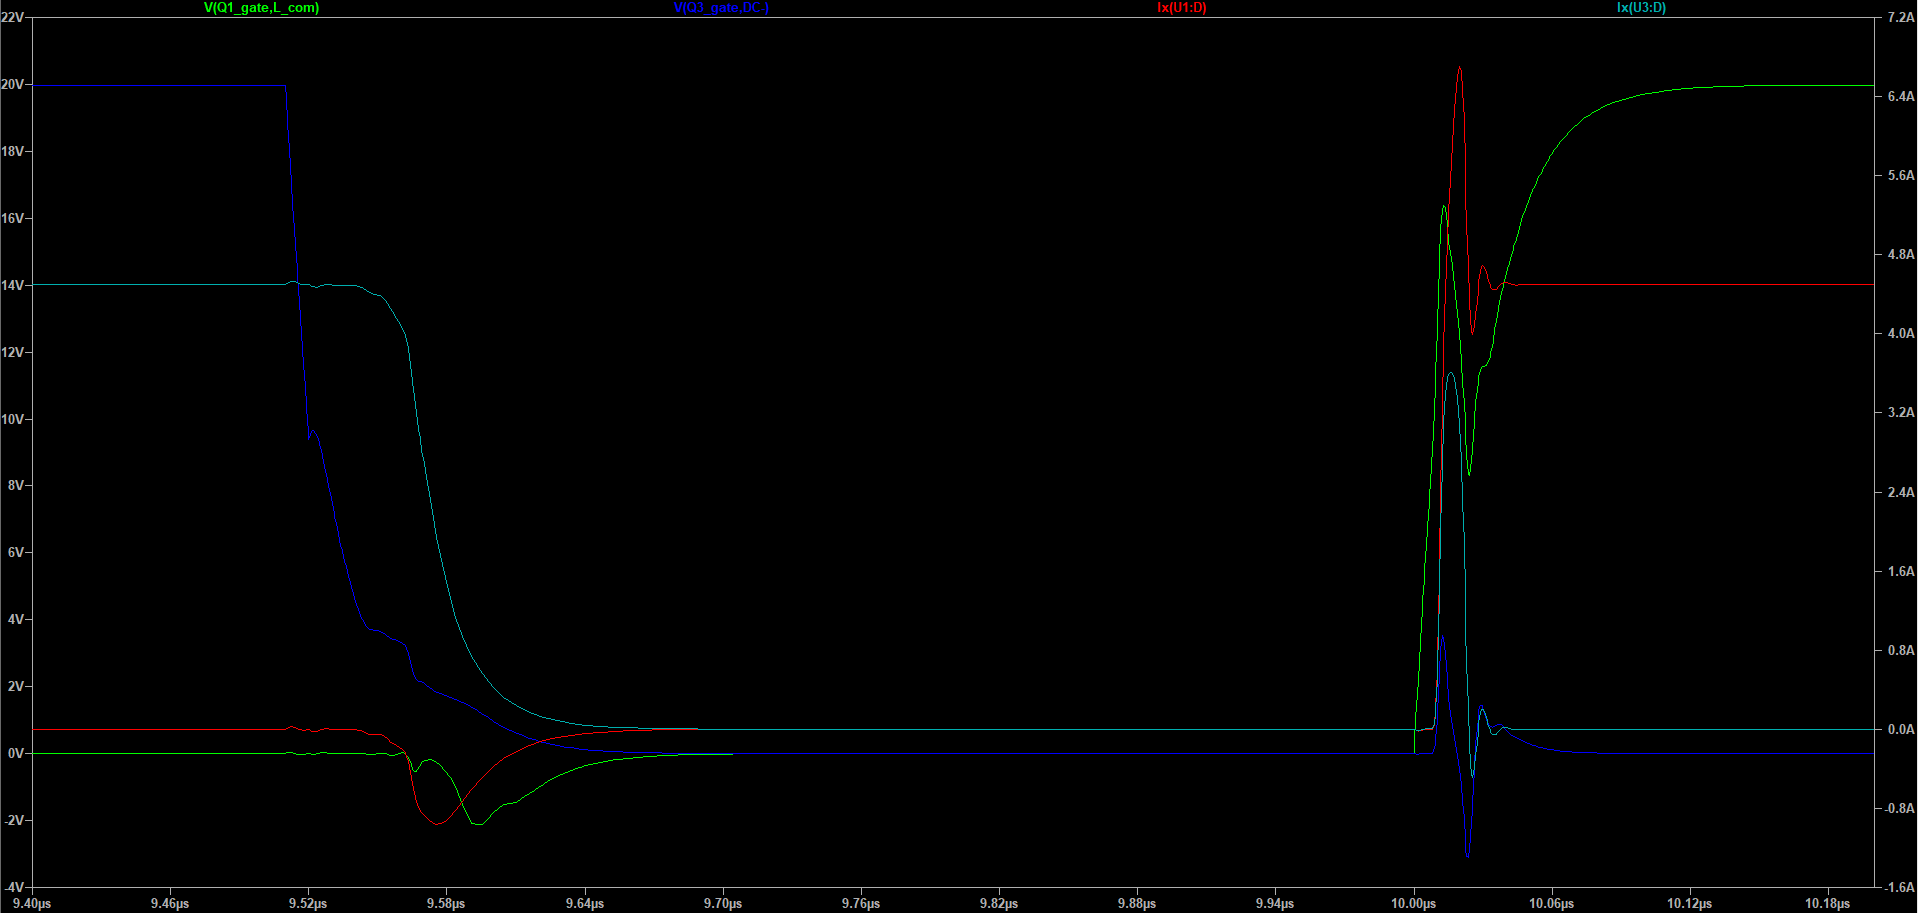
\includegraphics[width=\textwidth]{pictures/implementation/plain/plain_gates_3.PNG}
	\caption{Q3 turn off transient, gate voltages and drain currents}
	\label{fig:plain_gates_3}
\end{figure}

\begin{figure}[H]
	\centering
	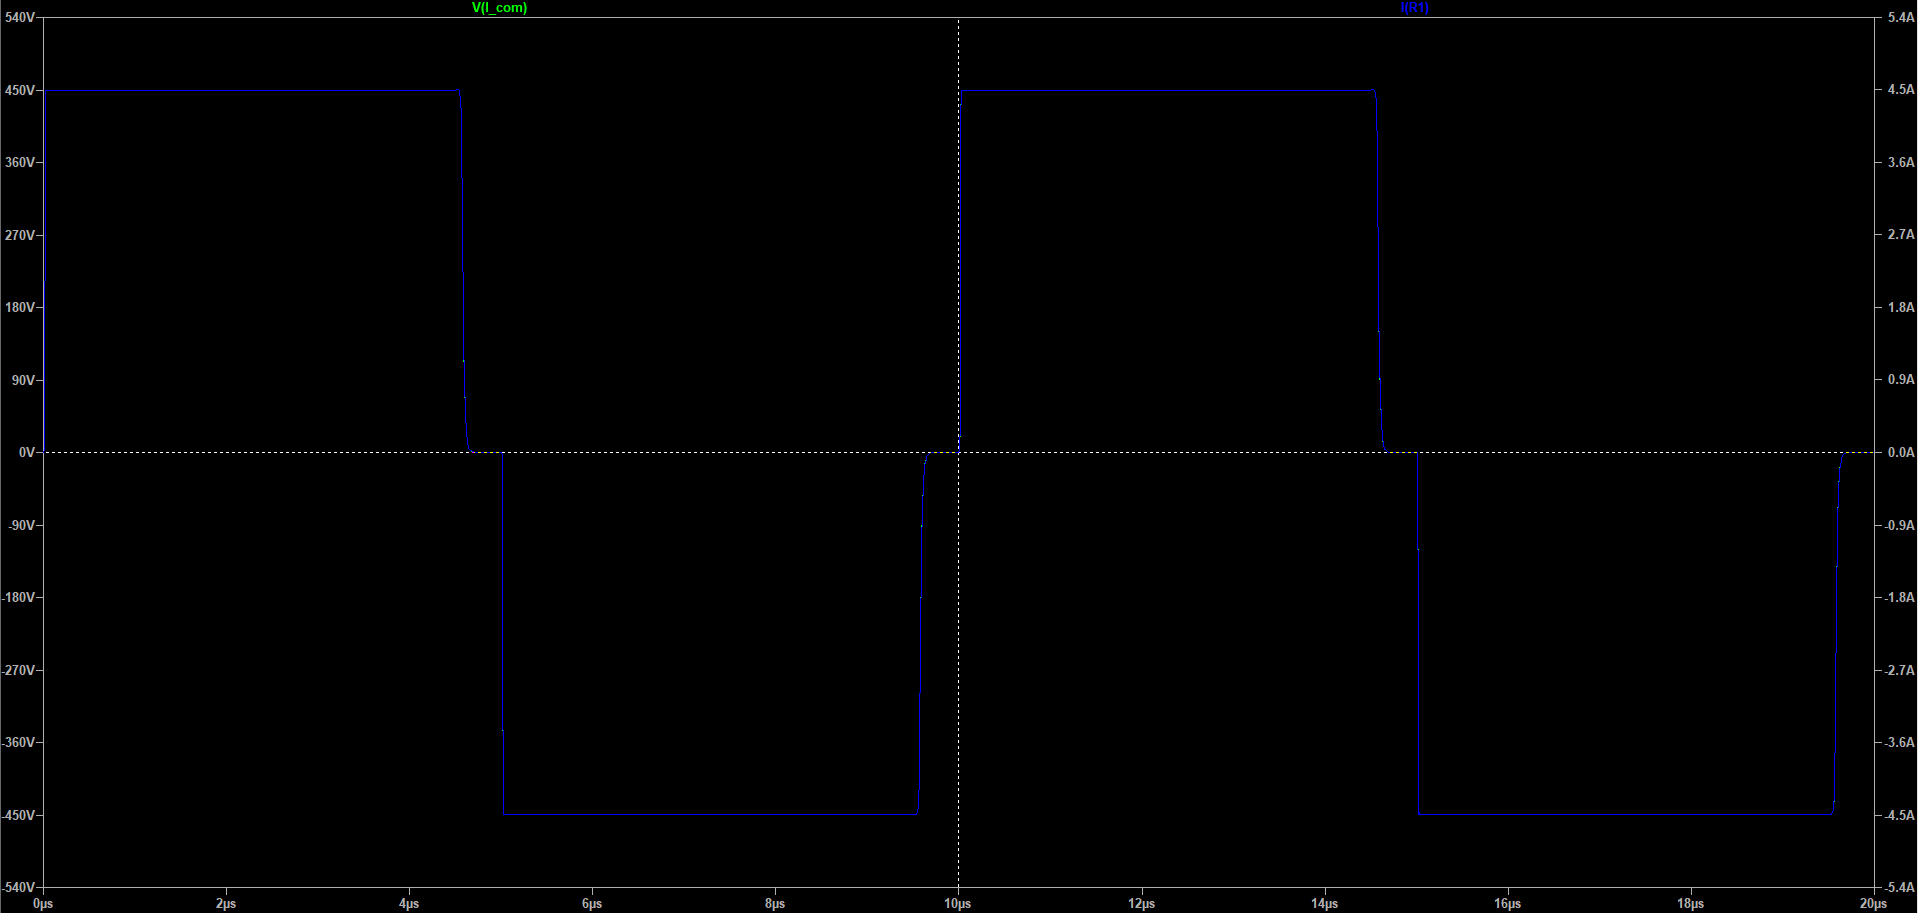
\includegraphics[width=\textwidth]{pictures/implementation/plain/plain_load.PNG}
	\caption{Voltage and current waveforms of the resistor overlap}
	\label{fig:plain_load}
\end{figure}

% Parasitic inductances
\subsection{Inductances}
\label{sec:inductances}

The step-by-step method of inductance extraction is found in Section \ref{sec:extraction}. This section deals with the reasoning behind investigating particular traces.

\begin{figure}[H]
	\centering
	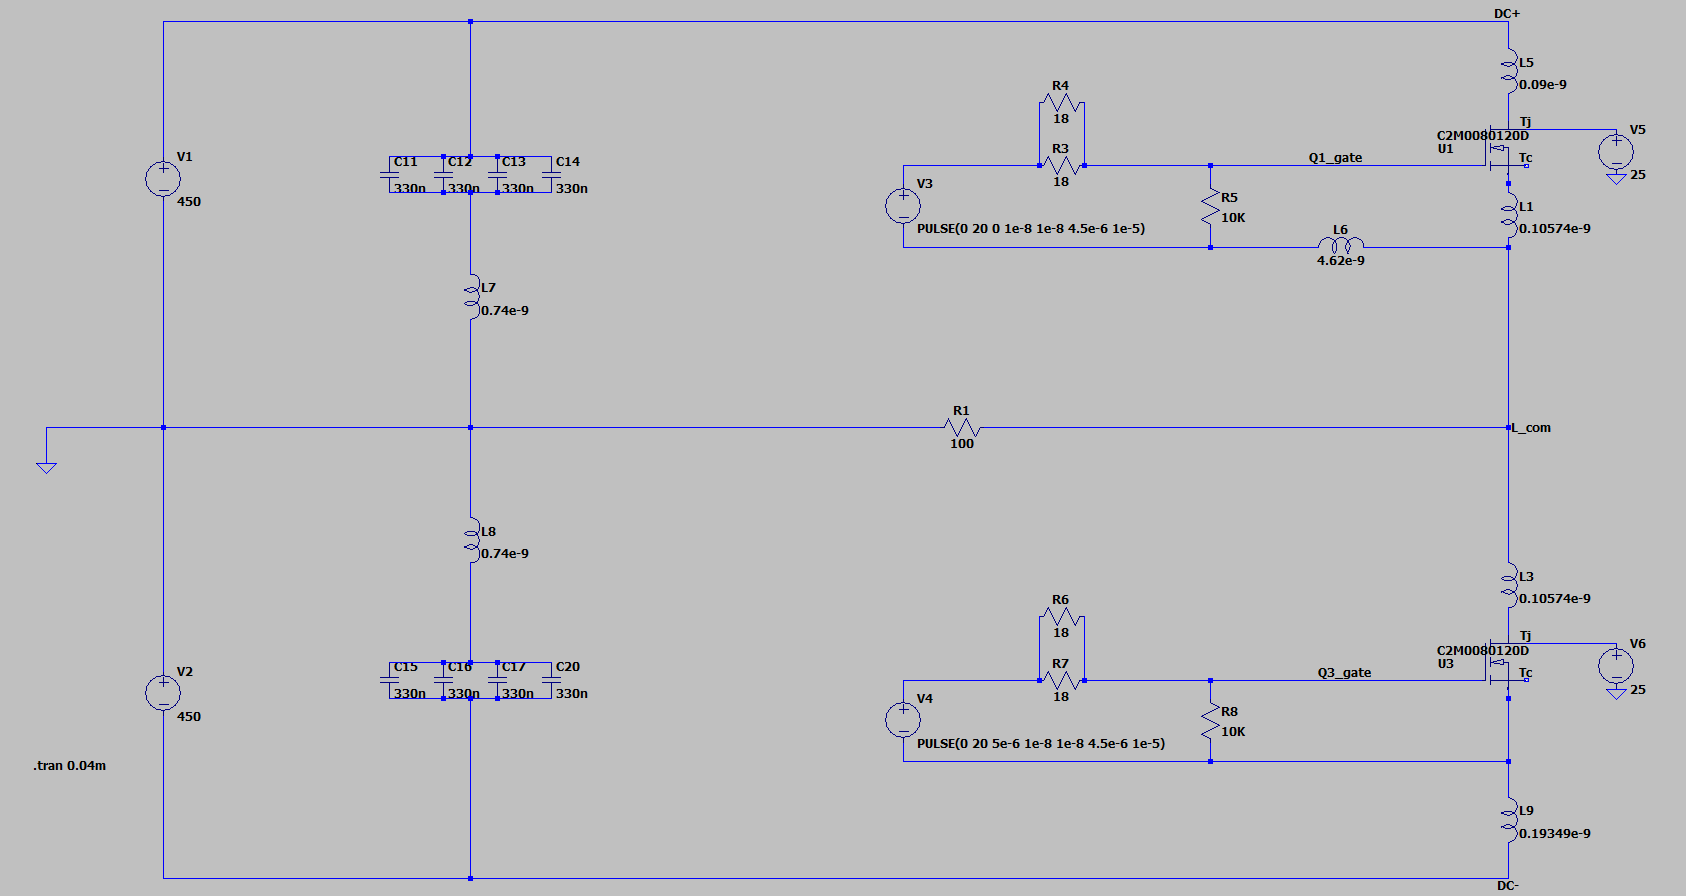
\includegraphics[width=\textwidth]{pictures/implementation/ind/spice_ind_1.PNG}
	\caption{Spice model with inductances}
	\label{fig:spice_ind}
\end{figure}

\subsubsection{Q1 drain}
\label{sec:Q1_drain}

The track between the drain terminal of Q1 and the capacitor bank C11-C12-C13-C14 is a part of interest. It is not only the DC+ power rail but Section \ref{sec:oscillators} details why the drain inductance is so critical. Section \ref{sec:extraction} details the position of the terminals in the layout. It is apparent that Q1 drain and the top of the capacitor bank is very close to each other on the layout and it manifests in a stray inductance value of $0.09 nH$ and negligible resistance.

\subsubsection{Q1 and Q3 gate}
\label{sec:q1_q3_gate}

Q1 and Q3 gate is driven via resistors very closely placed to the terminals. Their inductances proved to be extremely low, in the $pF$ order, therefore they were left out of the model. Figure \ref{fig:q1_gate} highlights the aforementioned distance at Q1. Q3 is symmetrical on the bottom side of the board.

\begin{figure}[H]
	\centering
	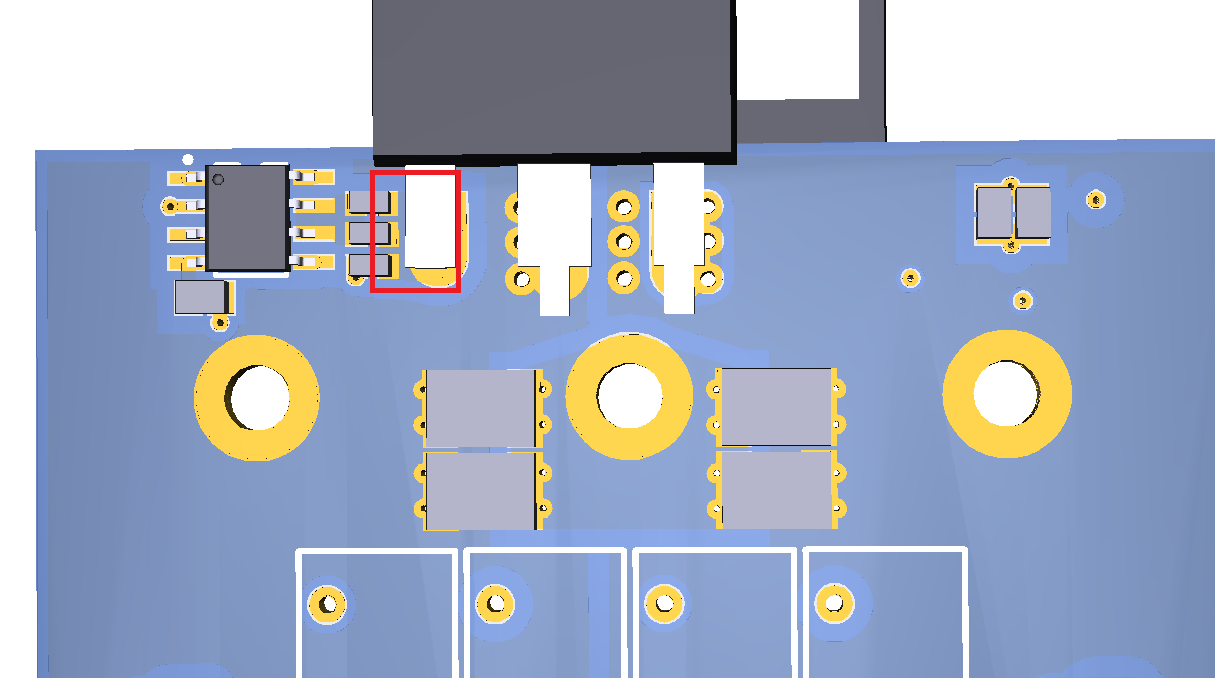
\includegraphics[width=\textwidth]{pictures/implementation/ind/Q1_gate.png}
	\caption{Distance between gate pin and drive line resistors}
	\label{fig:q1_gate}
\end{figure}

\subsubsection{Q1 source and Q3 drain}

The point L\_com in Figure \ref{fig:spice_ind} is a virtual point. It was inserted to connect the load nonexistent in the layout. It splits the L net in two, so for the sake of maintaining symmetry, the extracted inductance was also split in two. This yields a value of $0.106 nH$ for each of them with a practically negligible resistance of $0.00004 \ohm$.

\subsubsection{Q1 source and R5 lower pad}
\label{sec:q1_r5}

The gate signal return path is demonstrated in Figure \ref{fig:q1_r5}. The left small mark is the via to the bottom pad of R5. The total inductance extracted is $4.73 nH$. Since L1 is already represented in that loop, L6 got the value of $4.73 - 0.106 = 4.62 nH$. This may not matter much as L1 is about 2\% of the loop inductance but demonstrates the principle of partitioning a circuit.

\begin{figure}[H]
	\centering
	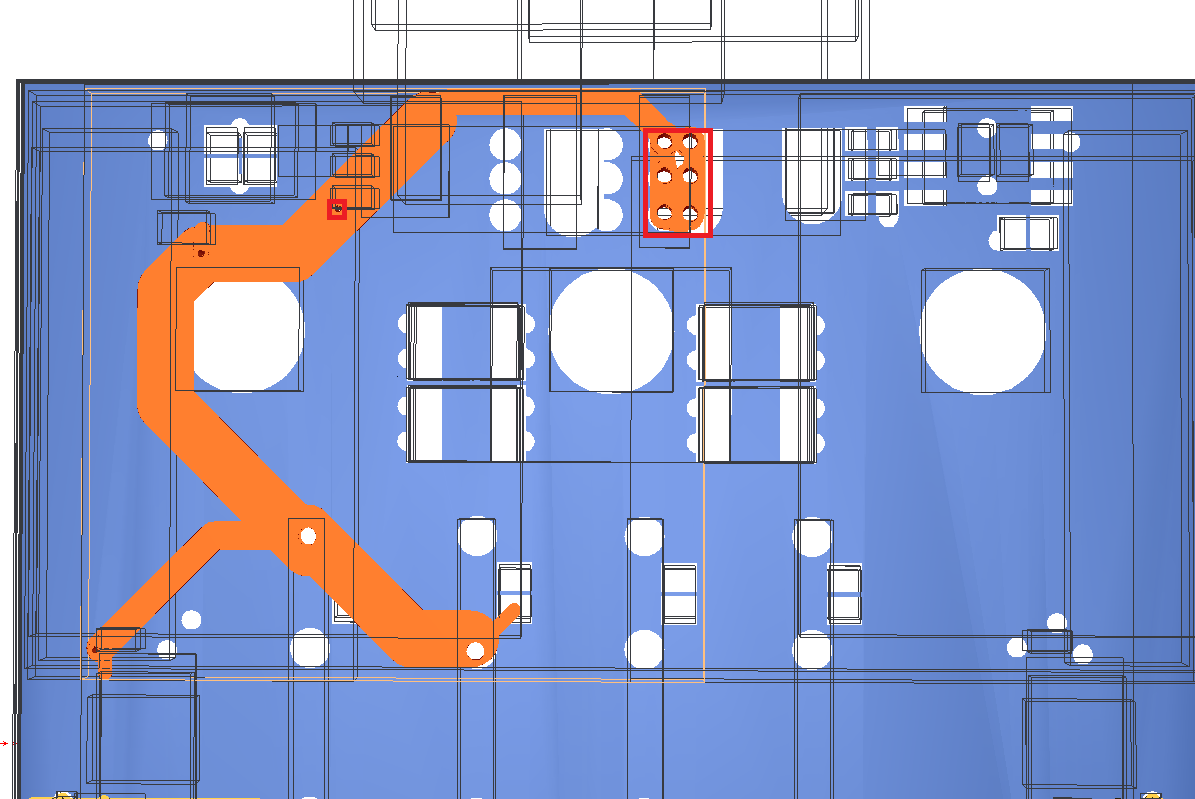
\includegraphics[width=\textwidth]{pictures/implementation/ind/q1_r5.png}
	\caption{Q1 gate signal return path}
	\label{fig:q1_r5}
\end{figure}

\subsubsection{Q3 source and DC-}
\label{sec:q3_source}

Inductance between the source of Q3 and the DC-rail is about as large as between $Q1_{source}$ and $Q3_{drain}$, $0.193 nH$.

\subsubsection{Capacitor banks}
\label{sec:cap_banks}

The inductance was split in two to accommodate the ground point of the symmetrical voltage sources. This yields $L7 = L8  = 0.74 nH$, with a resistance of $0.0013 \ohm$ for each.

\subsubsection{Waveforms}
\label{sec:ind_waveforms}

The simulated waveforms look plausible. Some cross-coupling can be seen at the moment of the switching but this is not enough to trigger false turn on-off cycles.

Figure \ref{fig:ind_gates_1} shows two whole cycles as an overview, Figure \ref{fig:ind_gates_2} shows the transient where $ Q1\ V_{GS}$ turns off, Figure \ref{fig:ind_gates_3} depicts the other end of that cycle. Figure \ref{fig:ind_load} demonstrates the voltage and current of the load.

\begin{figure}[H]
	\centering
	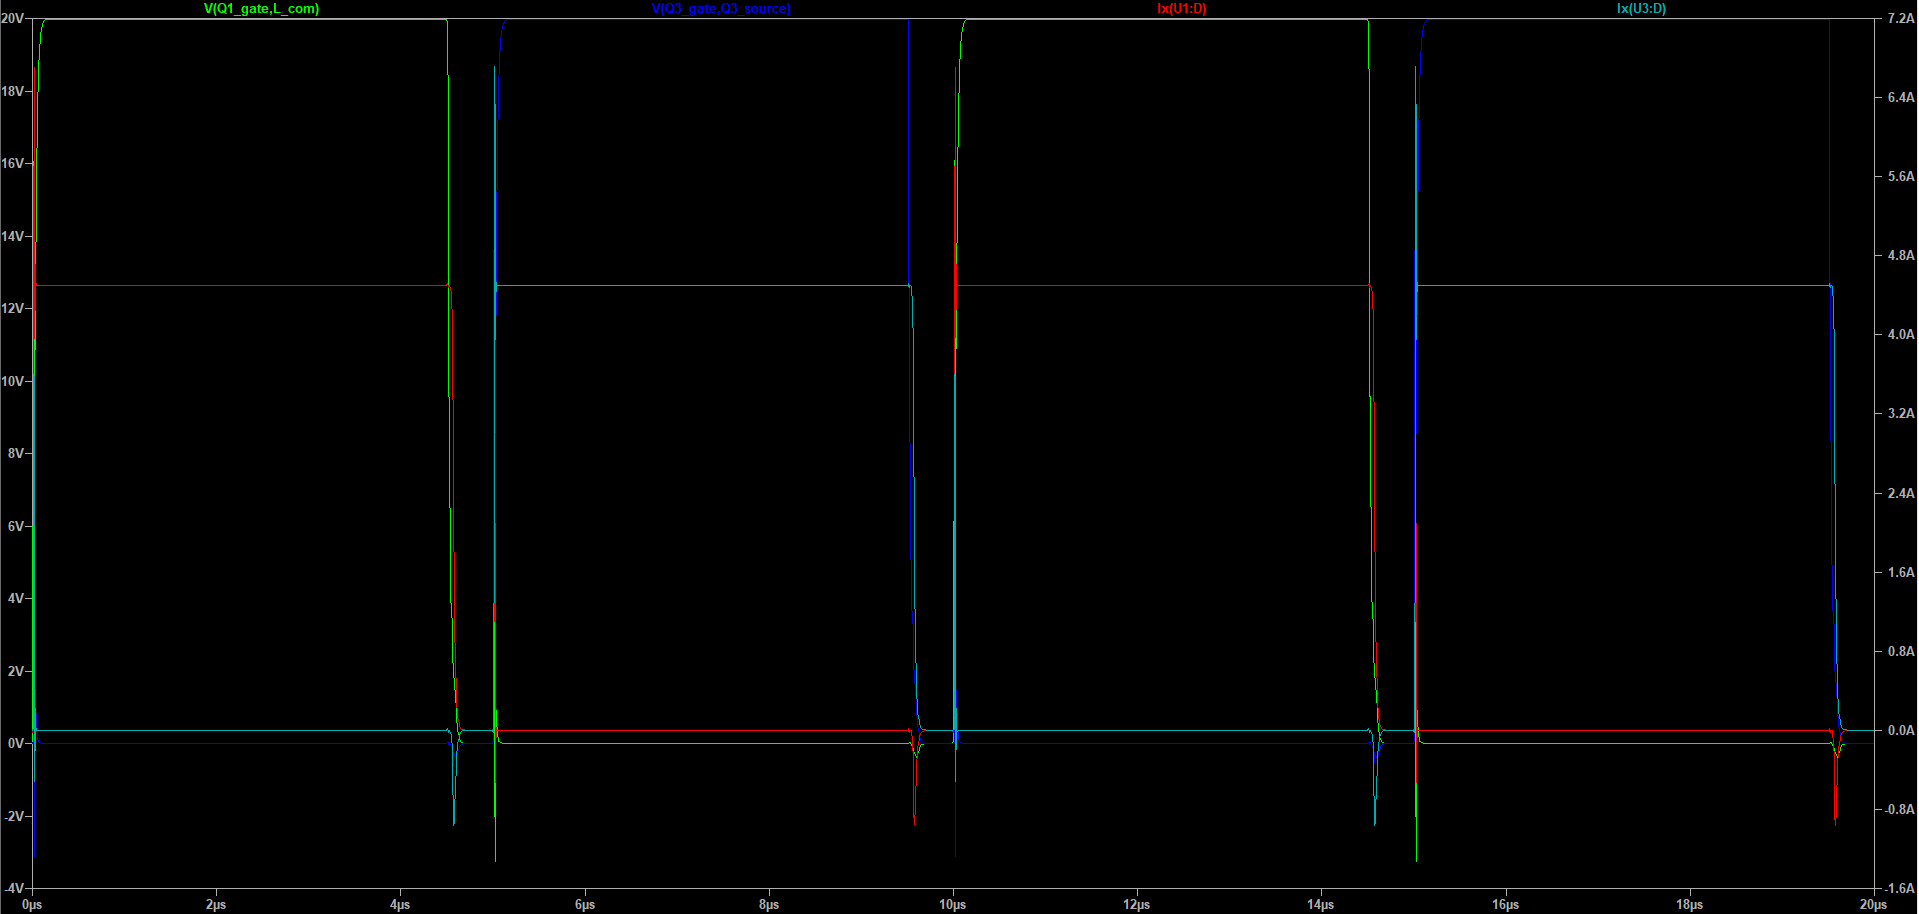
\includegraphics[width=\textwidth]{pictures/implementation/ind/ind_gates_1.PNG}
	\caption{Overview of the gate voltages and drain currents}
	\label{fig:ind_gates_1}
\end{figure}

\begin{figure}[H]
	\centering
	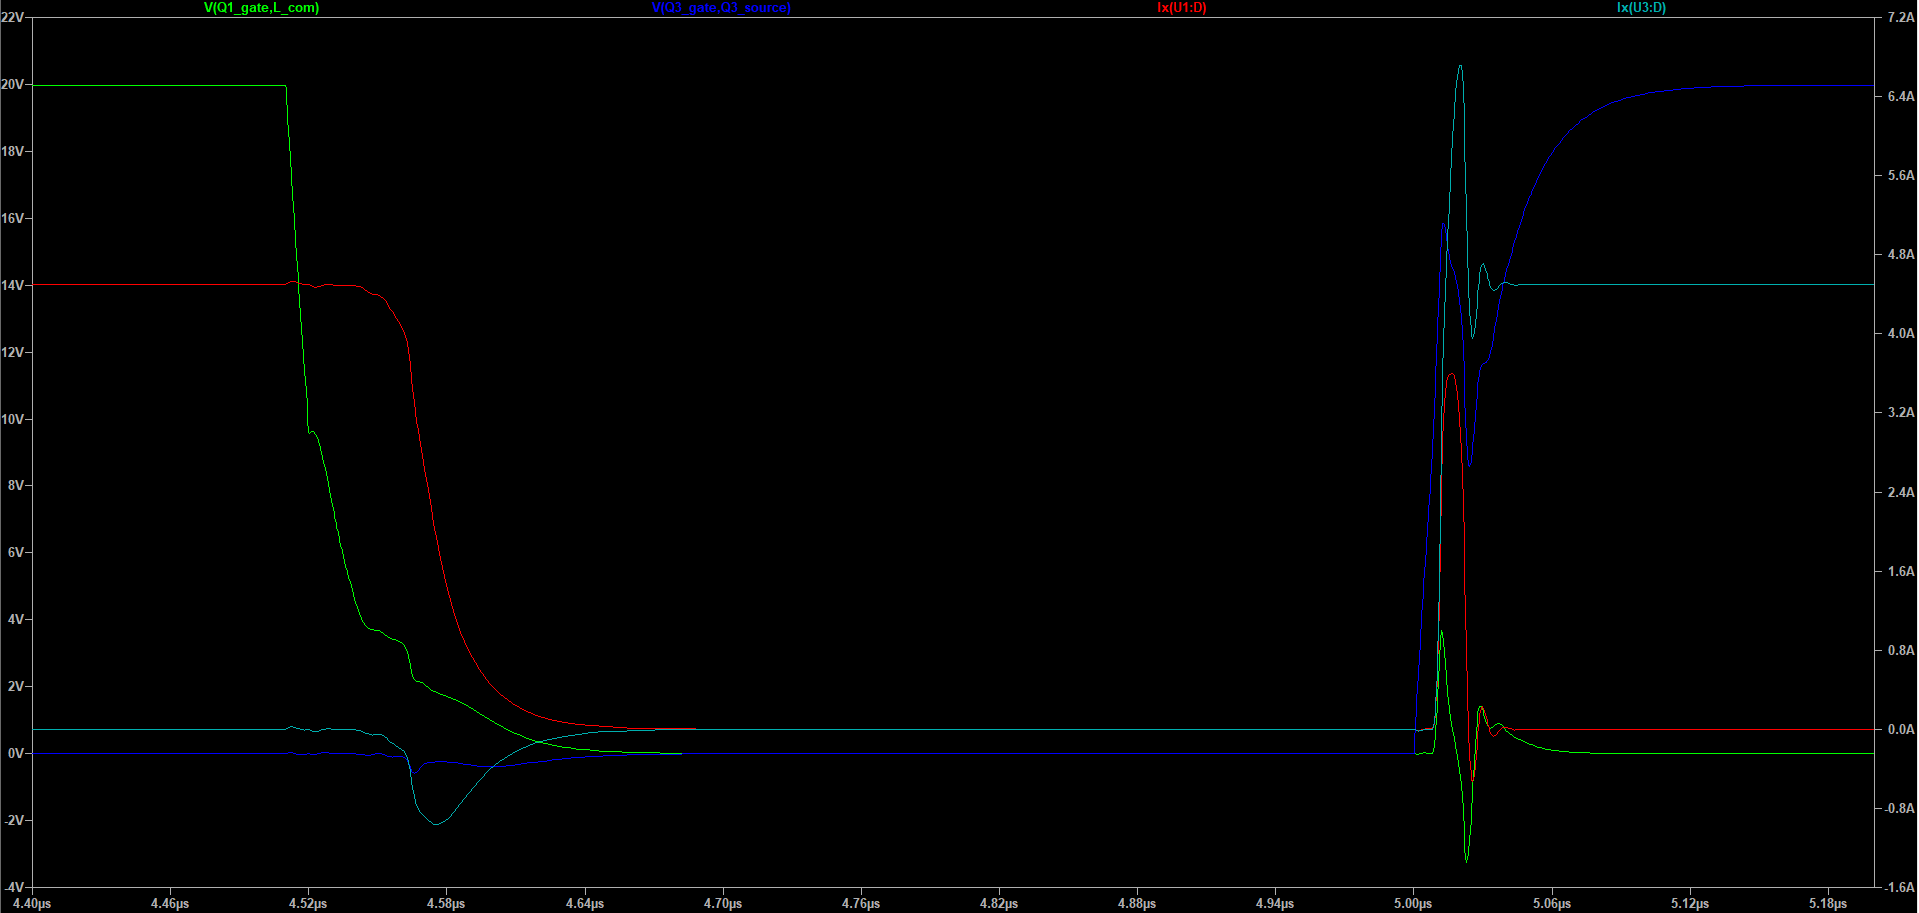
\includegraphics[width=\textwidth]{pictures/implementation/ind/ind_gates_2.PNG}
	\caption{Q1 turn off transient, gate voltages and drain currents}
	\label{fig:ind_gates_2}
\end{figure}

\begin{figure}[H]
	\centering
	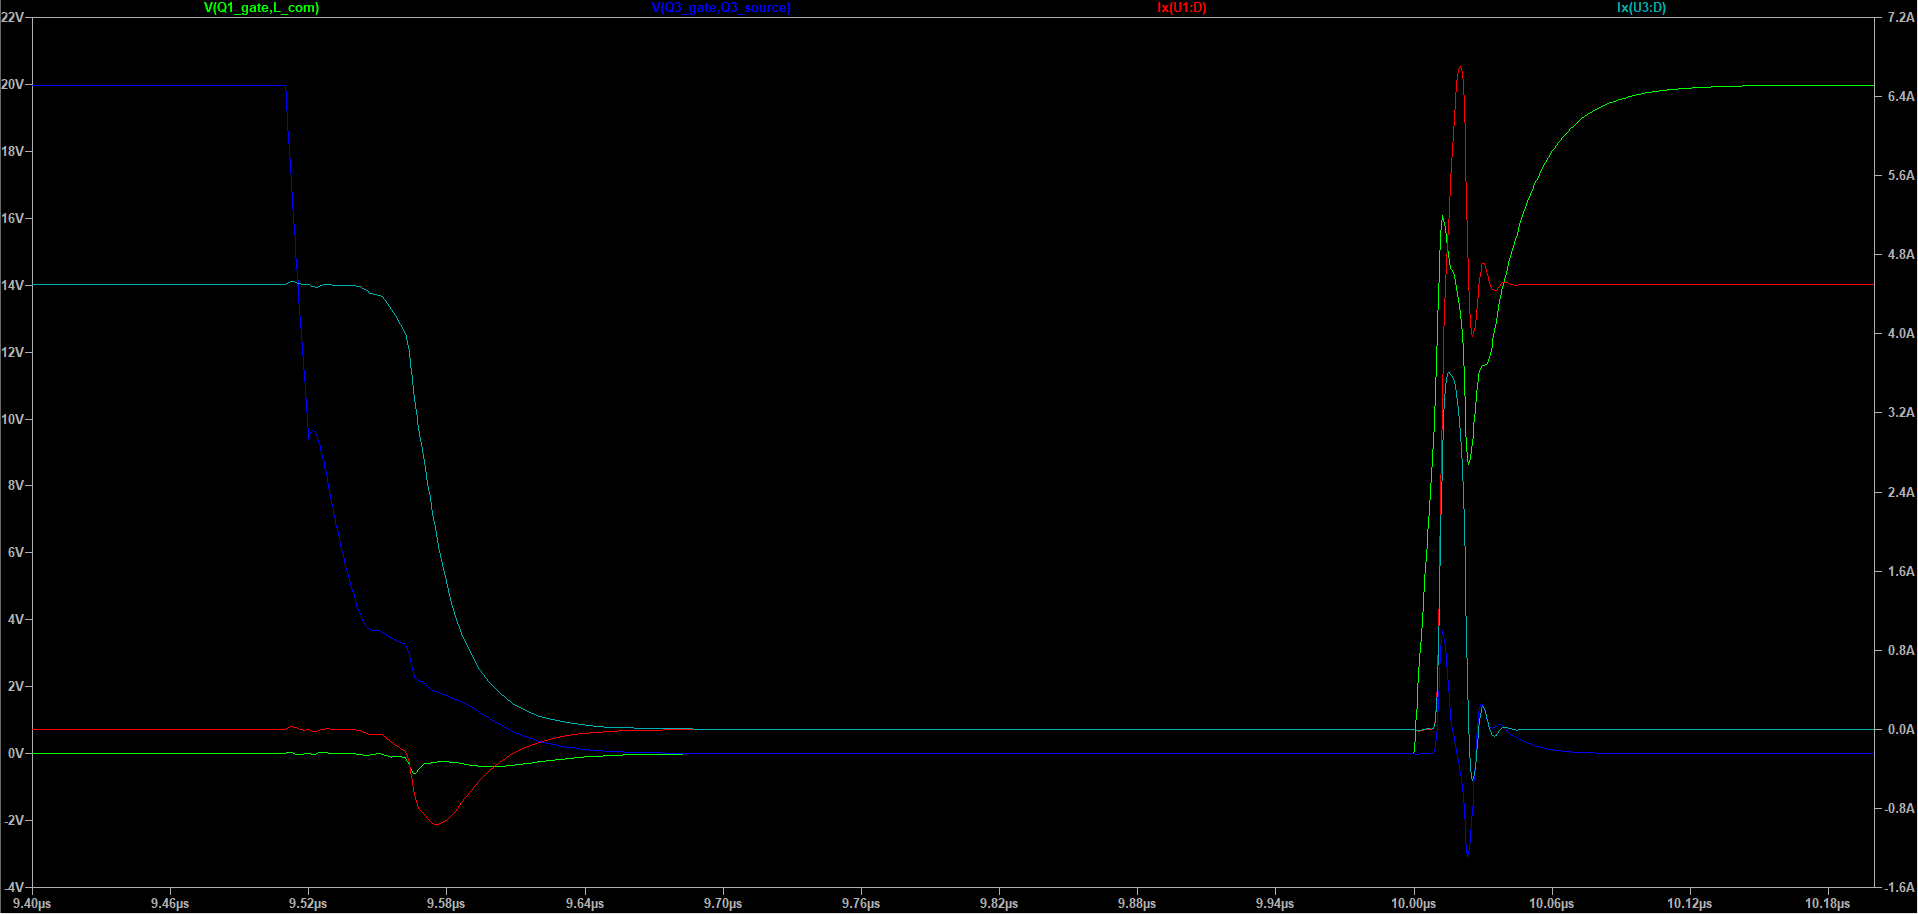
\includegraphics[width=\textwidth]{pictures/implementation/ind/ind_gates_3.PNG}
	\caption{Q3 turn off transient, gate voltages and drain currents}
	\label{fig:ind_gates_3}
\end{figure}

\begin{figure}[H]
	\centering
	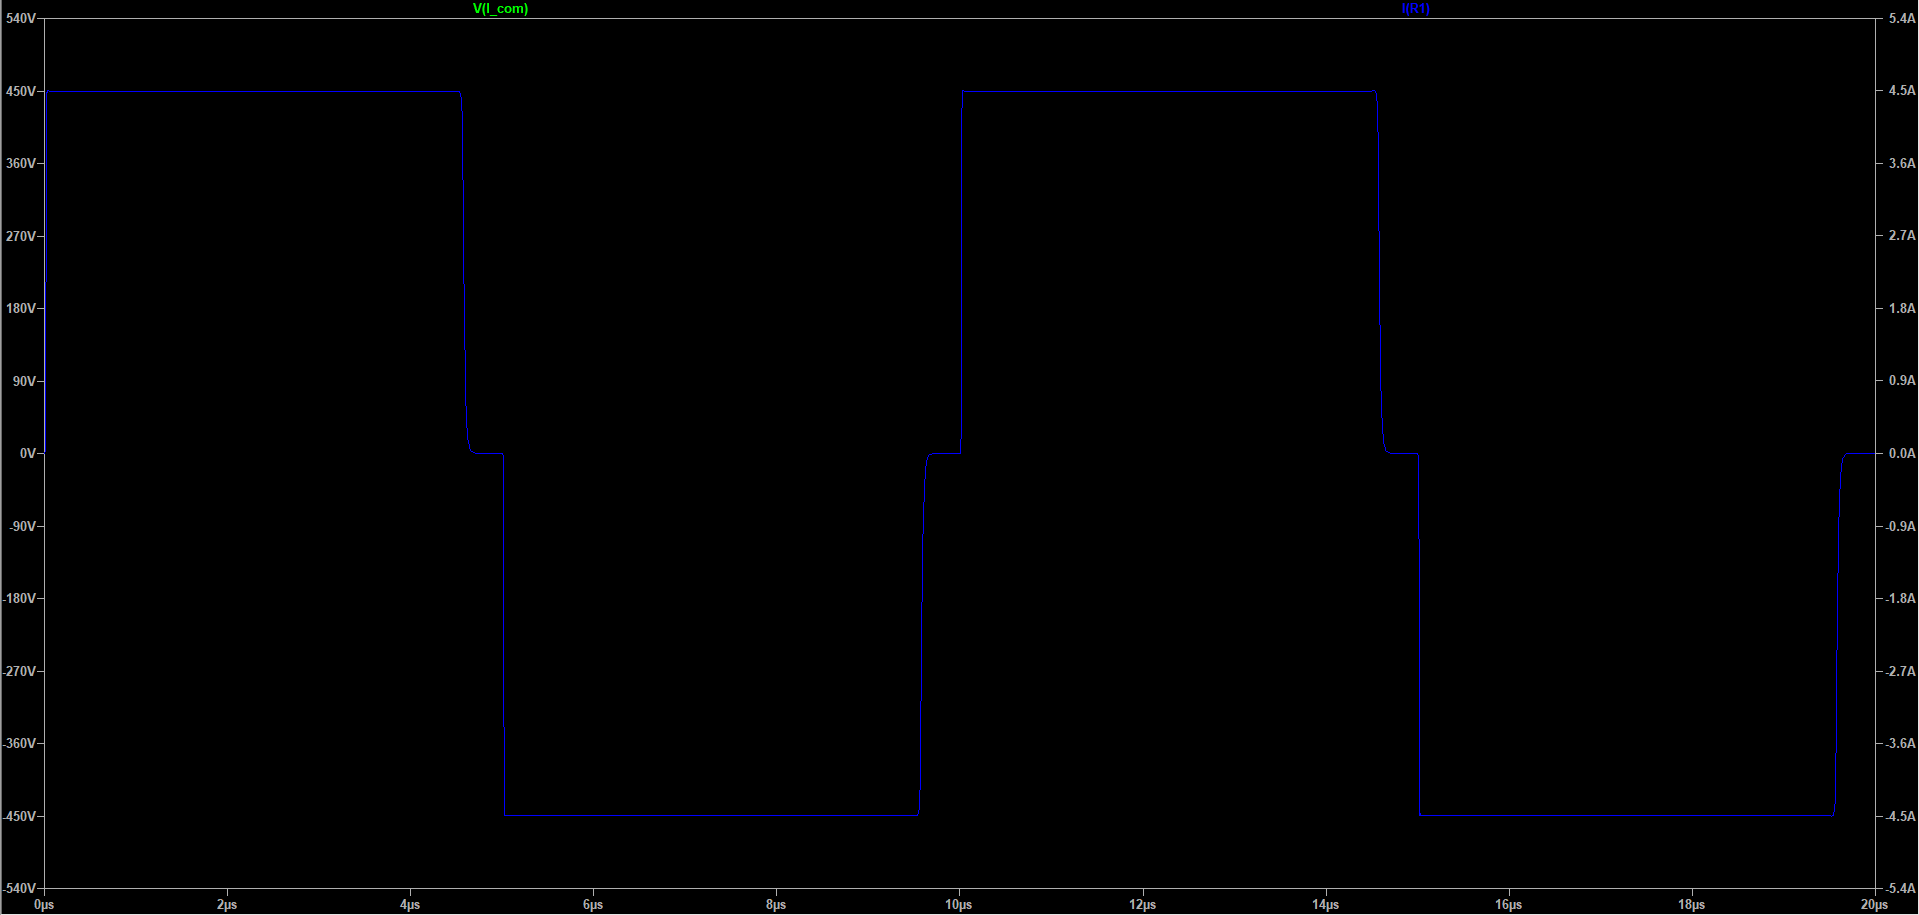
\includegraphics[width=\textwidth]{pictures/implementation/ind/ind_load.PNG}
	\caption{Voltage and current waveforms of the resistor overlap}
	\label{fig:ind_load}
\end{figure}

% Parasitic capacitances
\subsection{Capacitances}
\label{sec:capacitances}

Capacitances between pins of each MOSFET are interesting. They contribute to the potential oscillation circuit, so they should be minimized. The step-by-step method of capacitance extraction is found in Section \ref{sec:extraction}.

\begin{figure}[H]
	\centering
	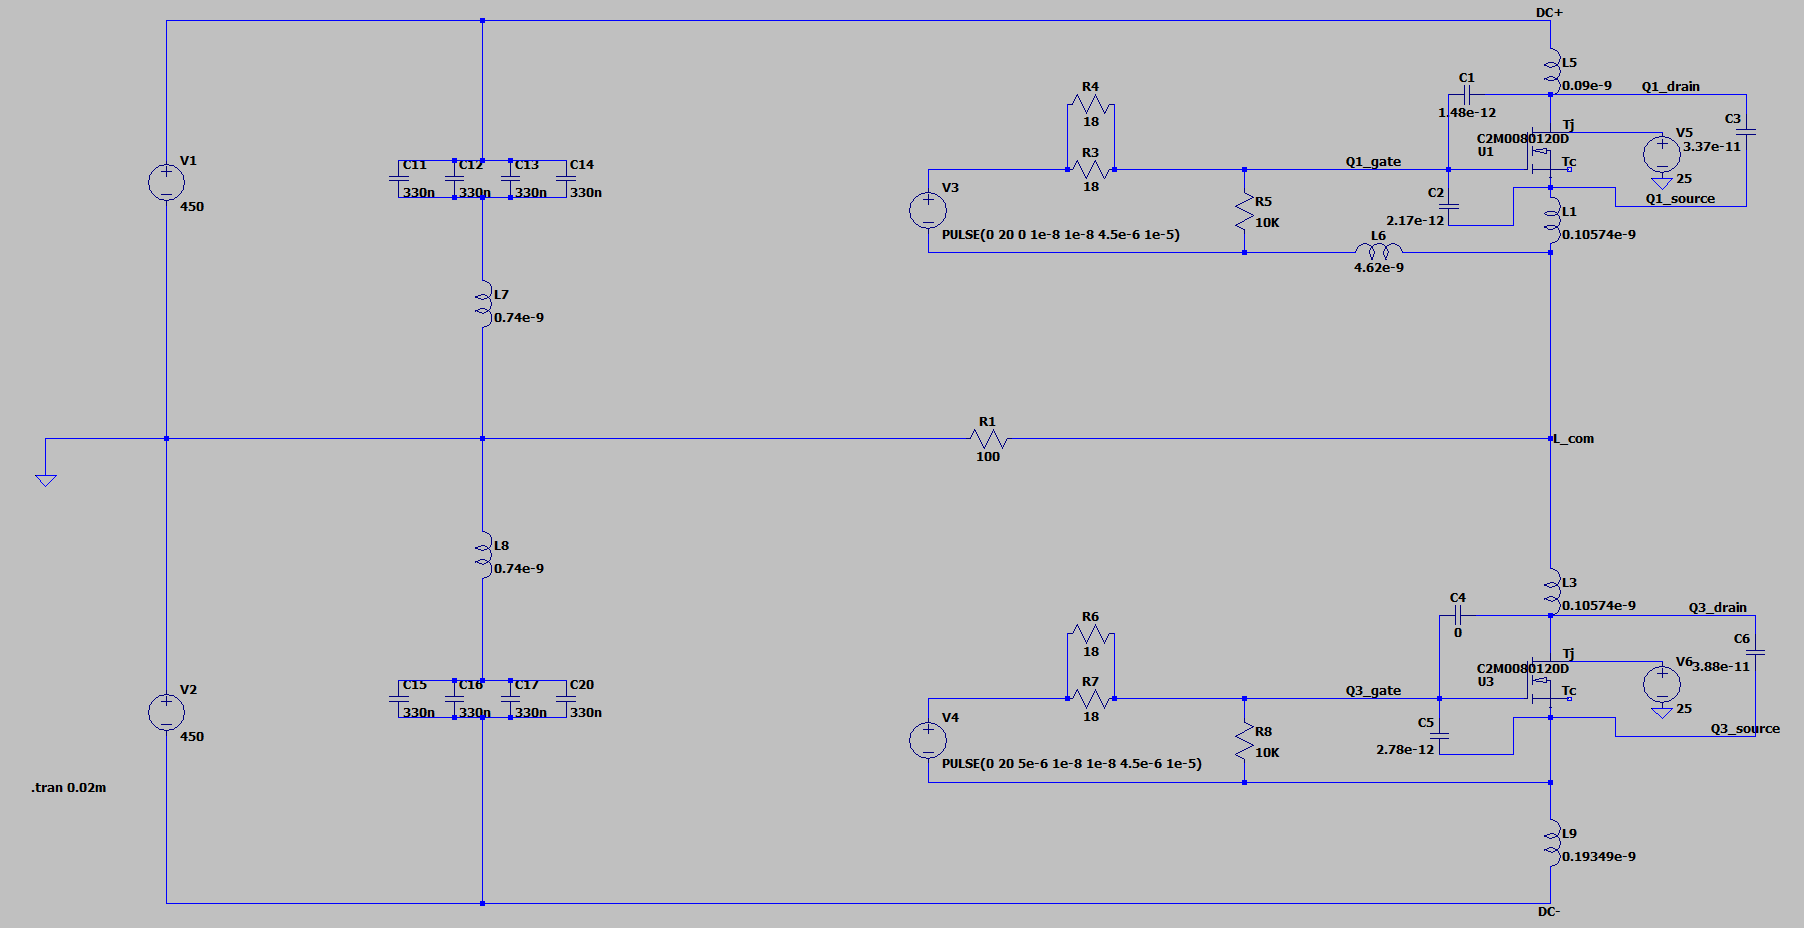
\includegraphics[width=\textwidth]{pictures/implementation/cap/spice_cap_1.PNG}
	\caption{Spice model with capacitances}
	\label{fig:spice_cap}
\end{figure}

\subsubsection{Q1 gate and drain}
\label{sec:q1_gate_drain}

The capacitance was extracted between the nets seen in Figure \ref{fig:cap_q1_g_d}. Its value of $1.48 pF$ is in the expected order of magnitude.

\begin{figure}[H]
	\centering
	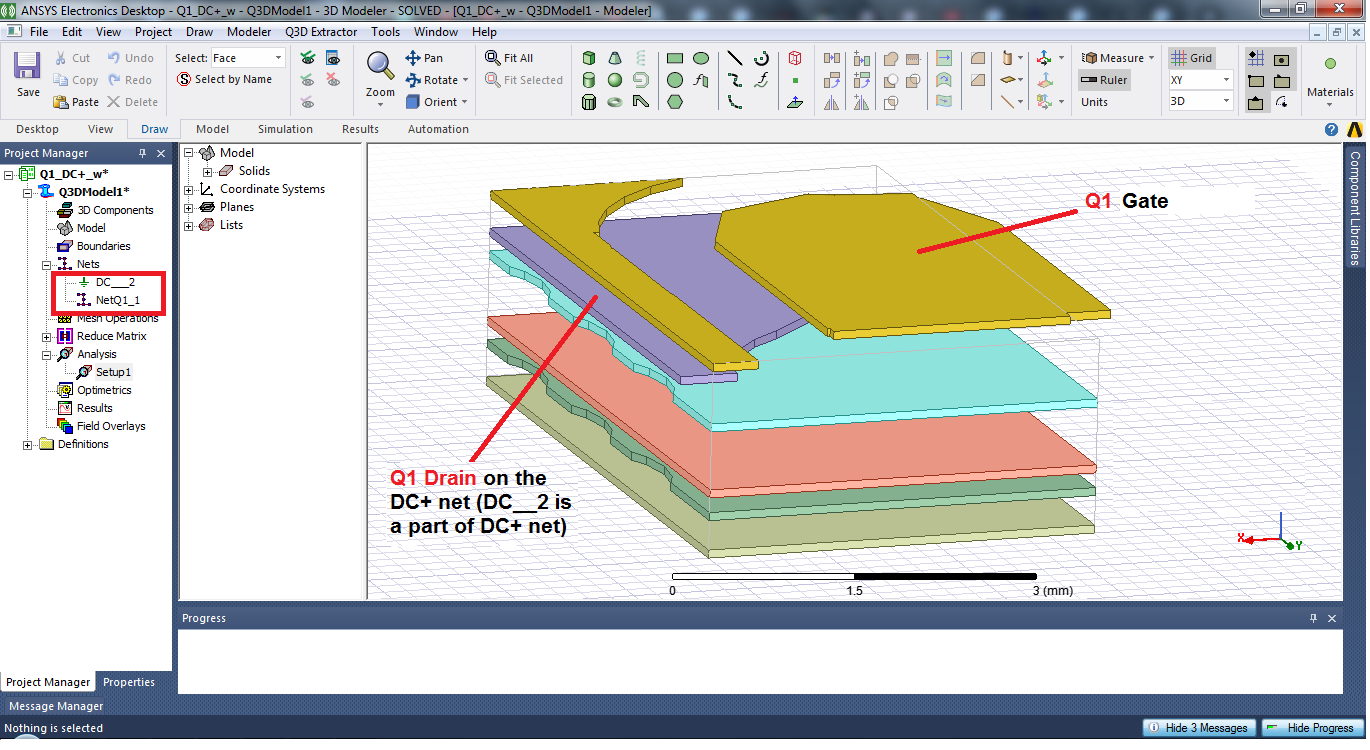
\includegraphics[width=\textwidth]{pictures/implementation/cap/cap_q1_g_d.PNG}
	\caption{The Q1-gate and Q1-drain net}
	\label{fig:cap_q1_g_d}
\end{figure}

\subsubsection{Q1 gate and source}
\label{sec:q1_gate_source}

The capacitance was extracted between the nets seen in Figure \ref{fig:cap_q1_g_s}. Its value of $2.17 pF$ is in the expected order of magnitude.

\begin{figure}[H]
	\centering
	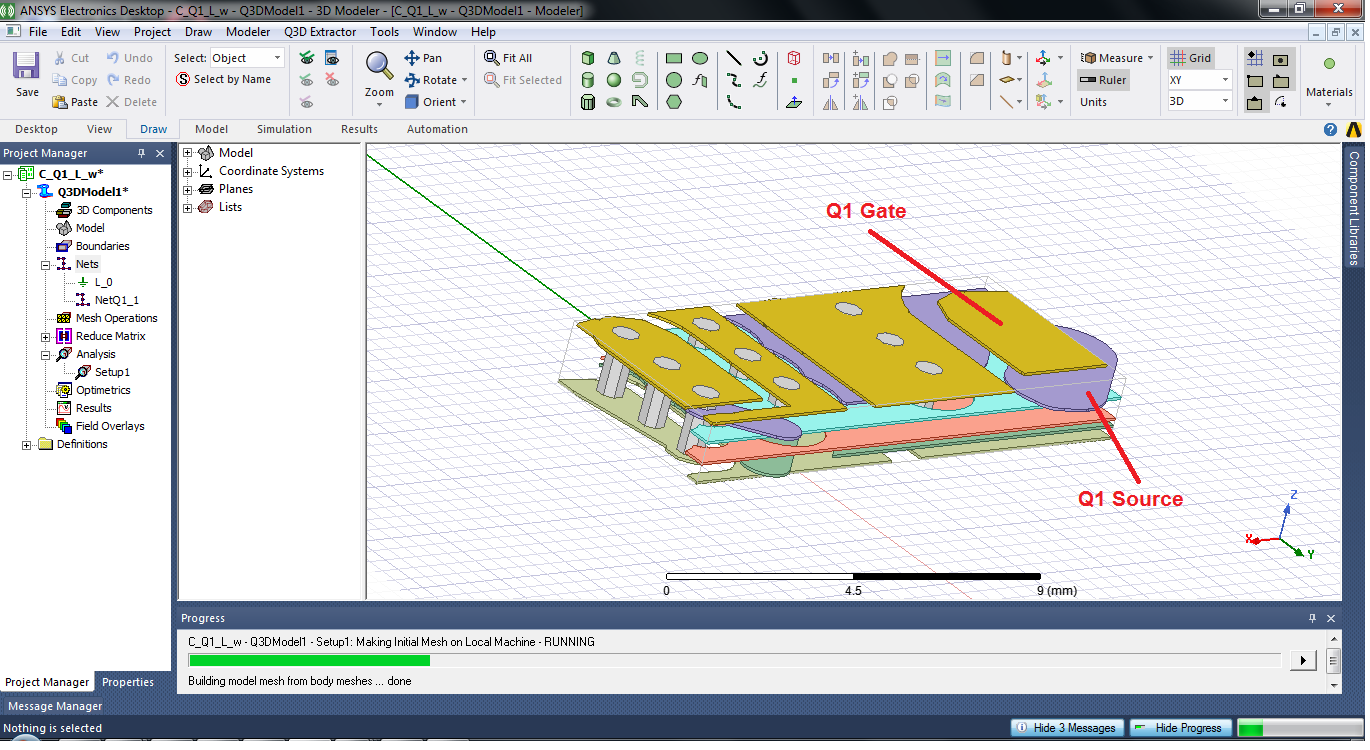
\includegraphics[width=\textwidth]{pictures/implementation/cap/cap_q1_g_s.PNG}
	\caption{The Q1-gate and Q1-source net}
	\label{fig:cap_q1_g_s}
\end{figure}

\subsubsection{Q1 drain and source}
\label{sec:q1_drain_source}

The capacitance was extracted between the nets seen in Figure \ref{fig:cap_q1_d_s}. Its value of $33.7 pF$ is in the expected order of magnitude.

\begin{figure}[H]
	\centering
	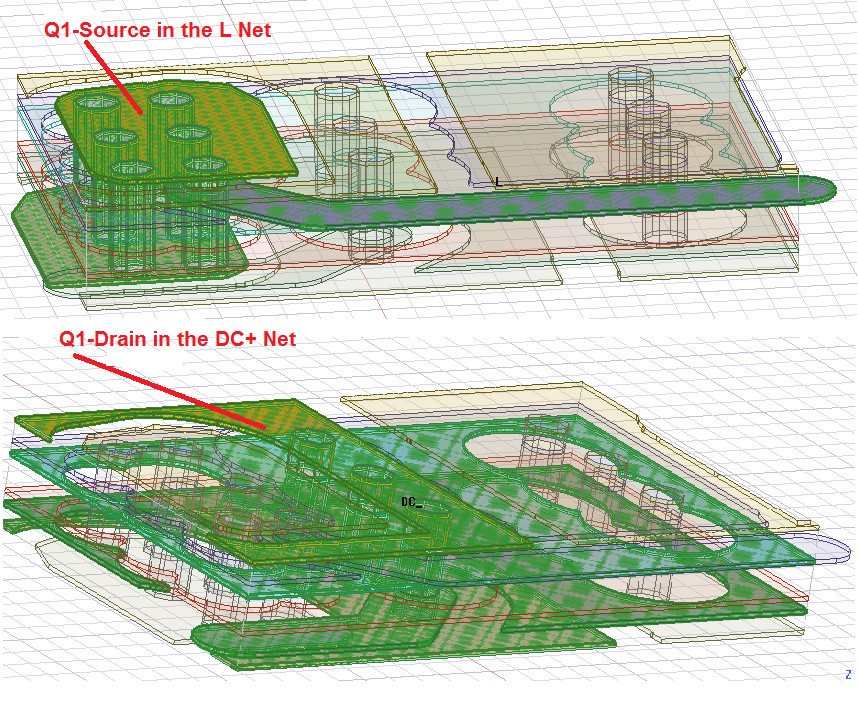
\includegraphics[width=\textwidth]{pictures/implementation/cap/cap_q1_d_s.PNG}
	\caption{The Q1-drain and Q1-source net}
	\label{fig:cap_q1_d_s}
\end{figure}

\subsubsection{Q3 gate and drain}
\label{sec:q3_gate_drain}

Capacitance was attempted to be extracted between the nets seen in Figure \ref{fig:cap_q3_g_d}. Since there is no coupling between them, there is no appreciable capacitance.

\begin{figure}[H]
	\centering
	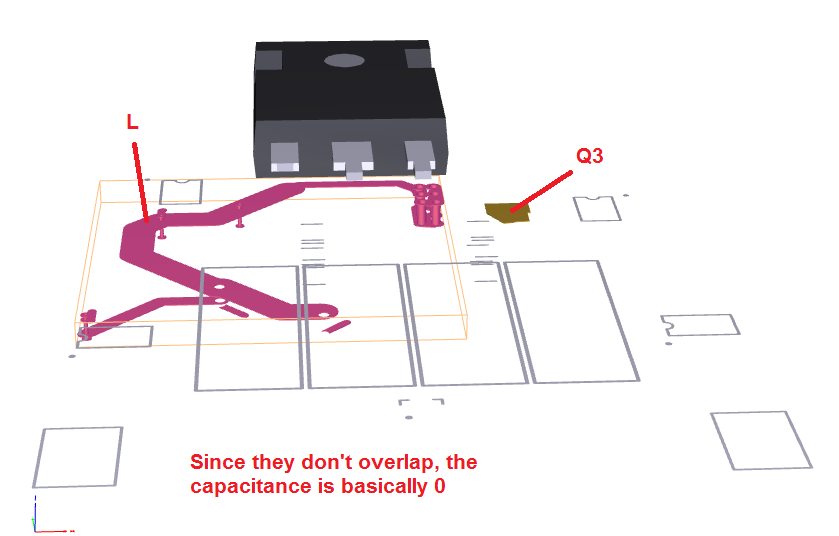
\includegraphics[width=\textwidth]{pictures/implementation/cap/cap_q3_g_d.PNG}
	\caption{The Q3-gate and Q3-drain net}
	\label{fig:cap_q3_g_d}
\end{figure}

\subsubsection{Q3 gate and source}
\label{sec:q3_gate_source}

The capacitance was extracted between the nets seen in Figure \ref{fig:cap_q3_g_s}. Its value of $2.78 pF$ is in the expected order of magnitude.

\begin{figure}[H]
	\centering
	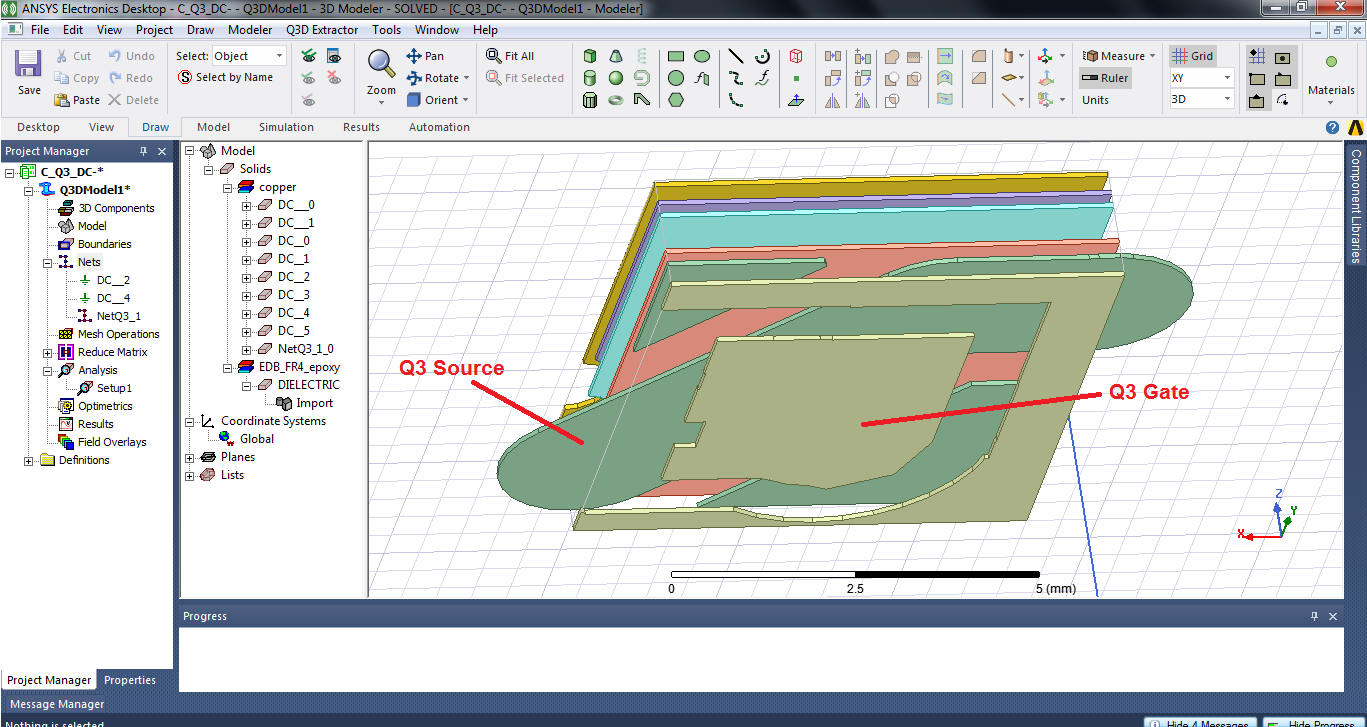
\includegraphics[width=\textwidth]{pictures/implementation/cap/cap_q3_g_s.PNG}
	\caption{The Q3-gate and Q3-source net}
	\label{fig:cap_q3_g_s}
\end{figure}

\subsubsection{Q3 drain and source}
\label{sec:q3_drain_source}

The capacitance was extracted between the nets seen in Figure \ref{fig:cap_q3_d_s}. Its value of $38.8 pF$ is in the expected order of magnitude.

\begin{figure}[H]
	\centering
	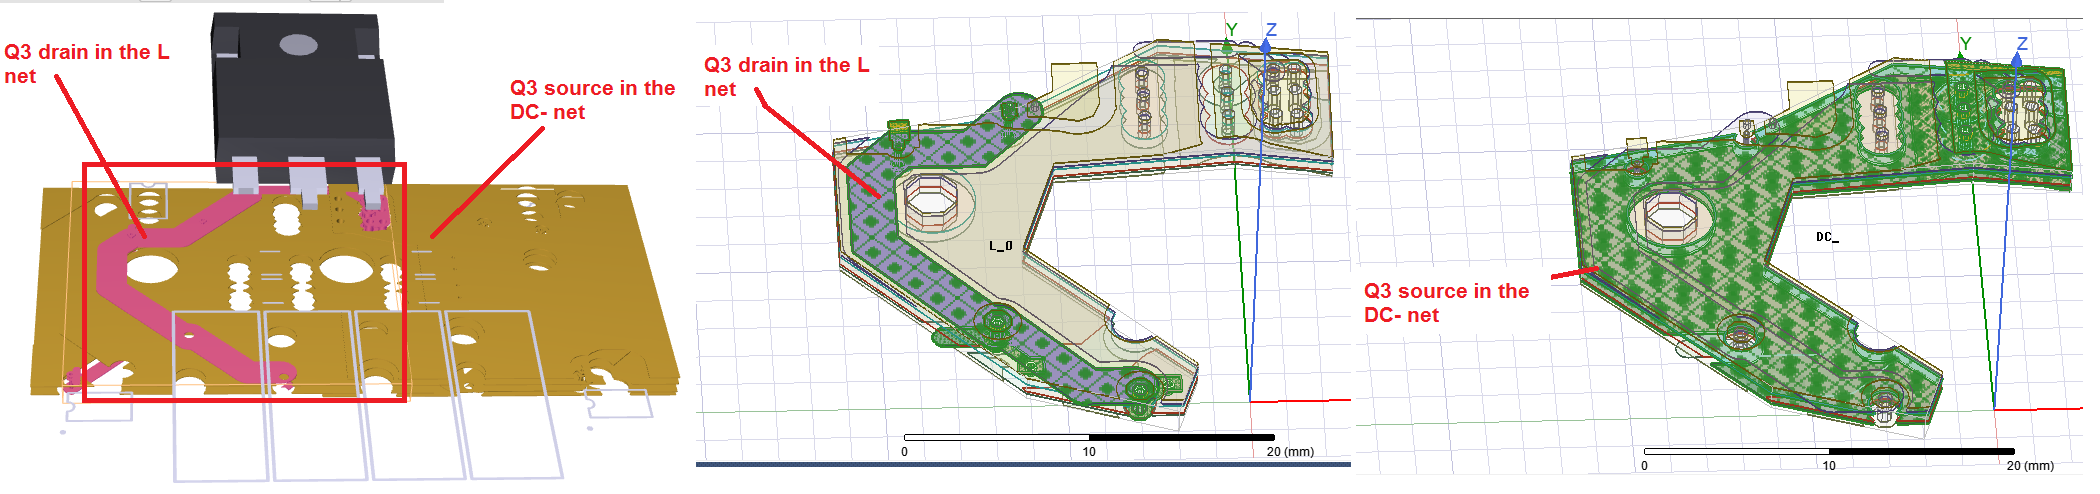
\includegraphics[width=\textwidth]{pictures/implementation/cap/cap_q3_d_s.PNG}
	\caption{The Q3-drain and Q3-source net}
	\label{fig:cap_q3_d_s}
\end{figure}


\subsubsection{Waveforms}
\label{sec:cap_waveforms}

The simulated waveforms look plausible. Some cross-coupling can be seen at the moment of the switching but this is not enough to trigger false turn on-off cycles.

Figure \ref{fig:cap_gates_1} shows two whole cycles as an overview, Figure \ref{fig:cap_gates_2} shows the transient where $V_{GS1}$ turns off, Figure \ref{fig:cap_gates_3} depicts the other end of that cycle. Figure \ref{fig:cap_load} demonstrates the voltage and current of the load.

\begin{figure}[H]
	\centering
	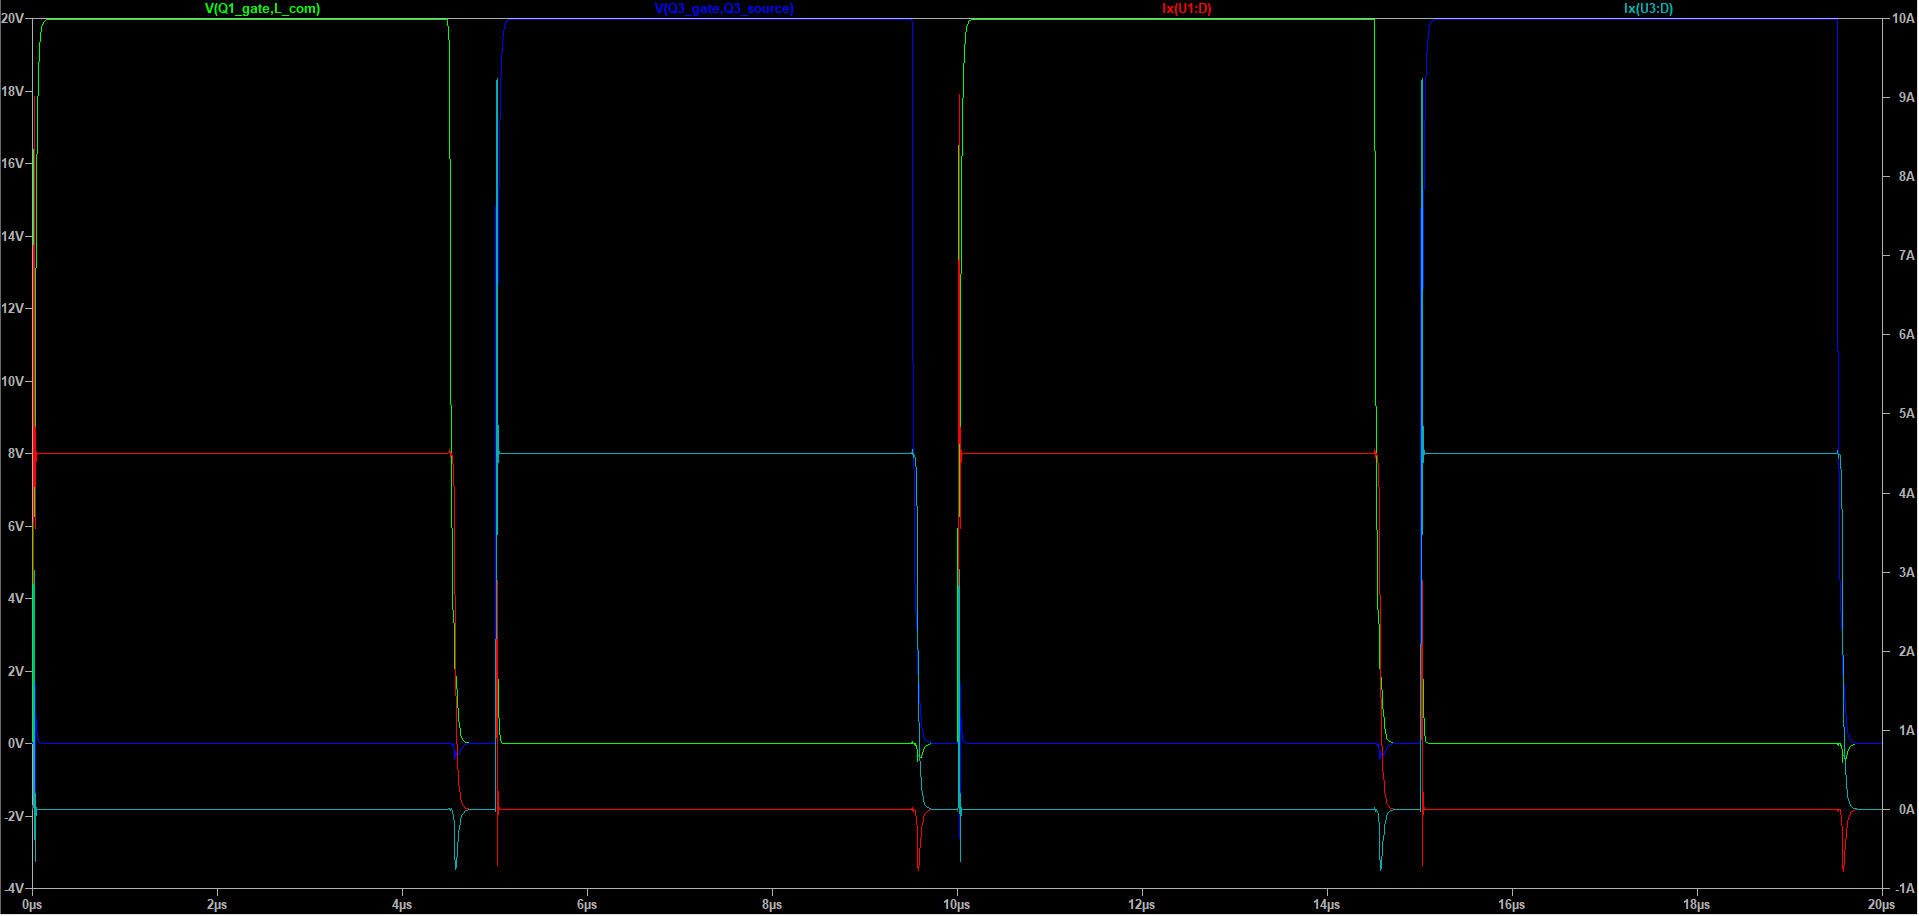
\includegraphics[width=\textwidth]{pictures/implementation/cap/cap_gates_1.PNG}
	\caption{Overview of the gate voltages and drain currents}
	\label{fig:cap_gates_1}
\end{figure}

\begin{figure}[H]
	\centering
	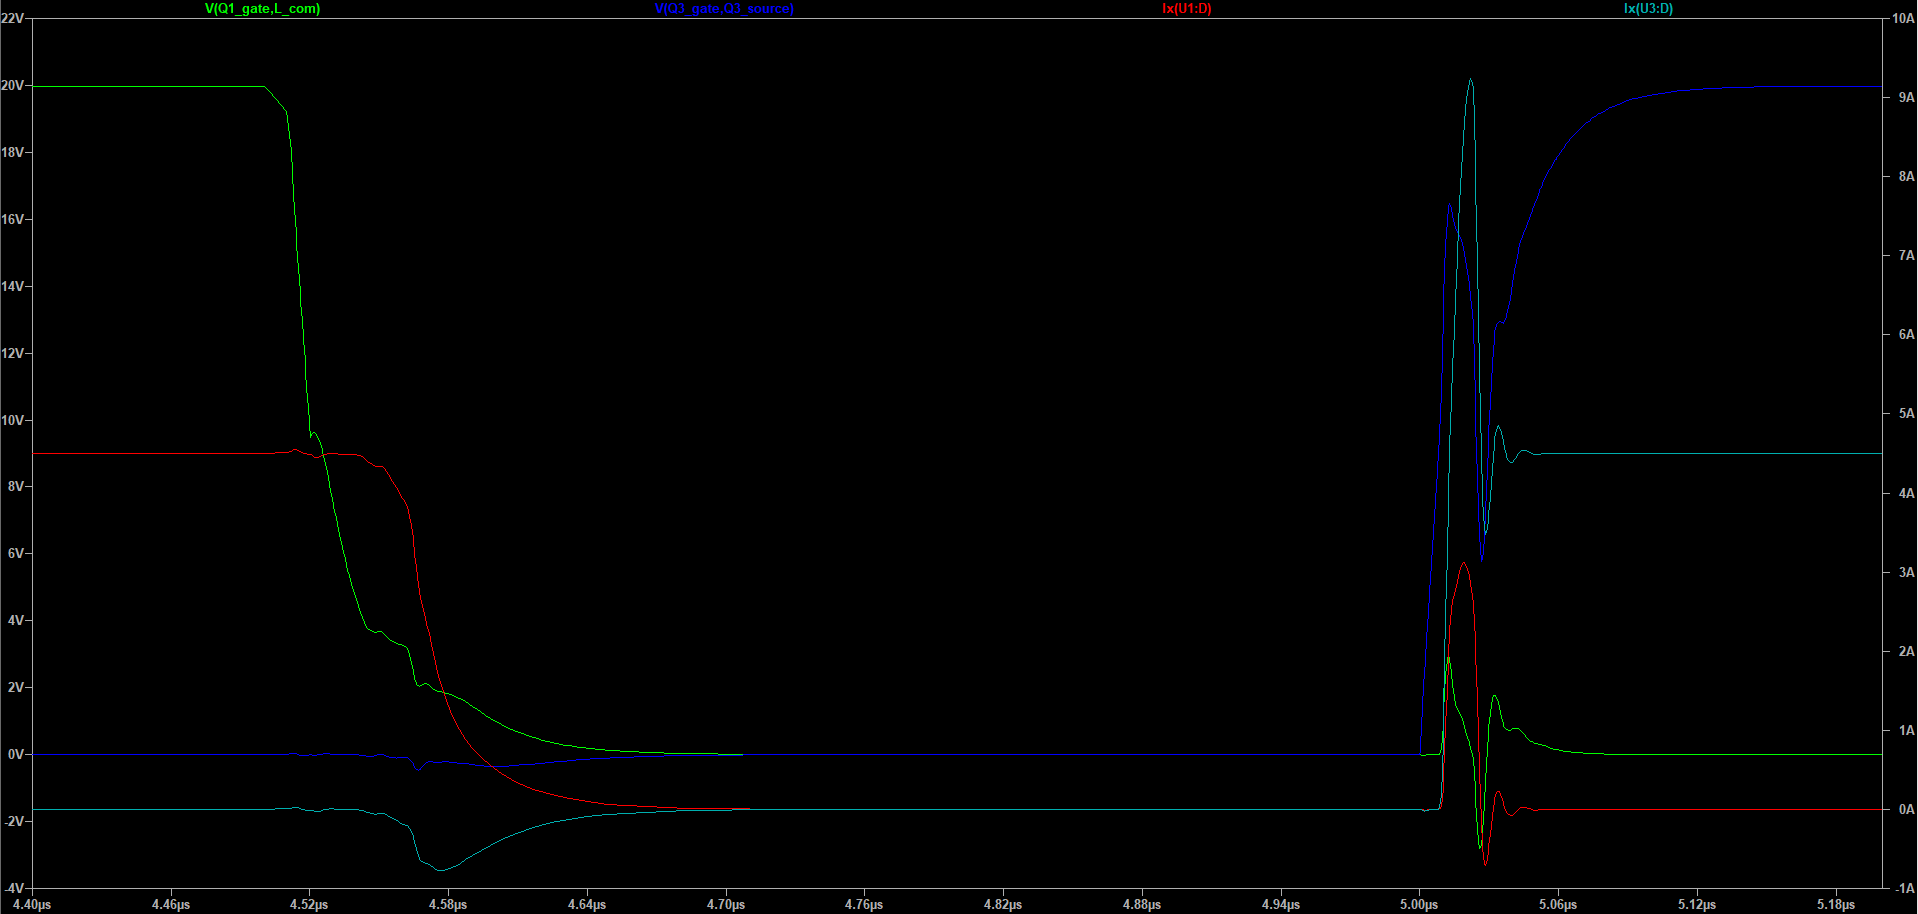
\includegraphics[width=\textwidth]{pictures/implementation/cap/cap_gates_2.PNG}
	\caption{Q1 turn off transient, gate voltages and drain currents}
	\label{fig:cap_gates_2}
\end{figure}

\begin{figure}[H]
	\centering
	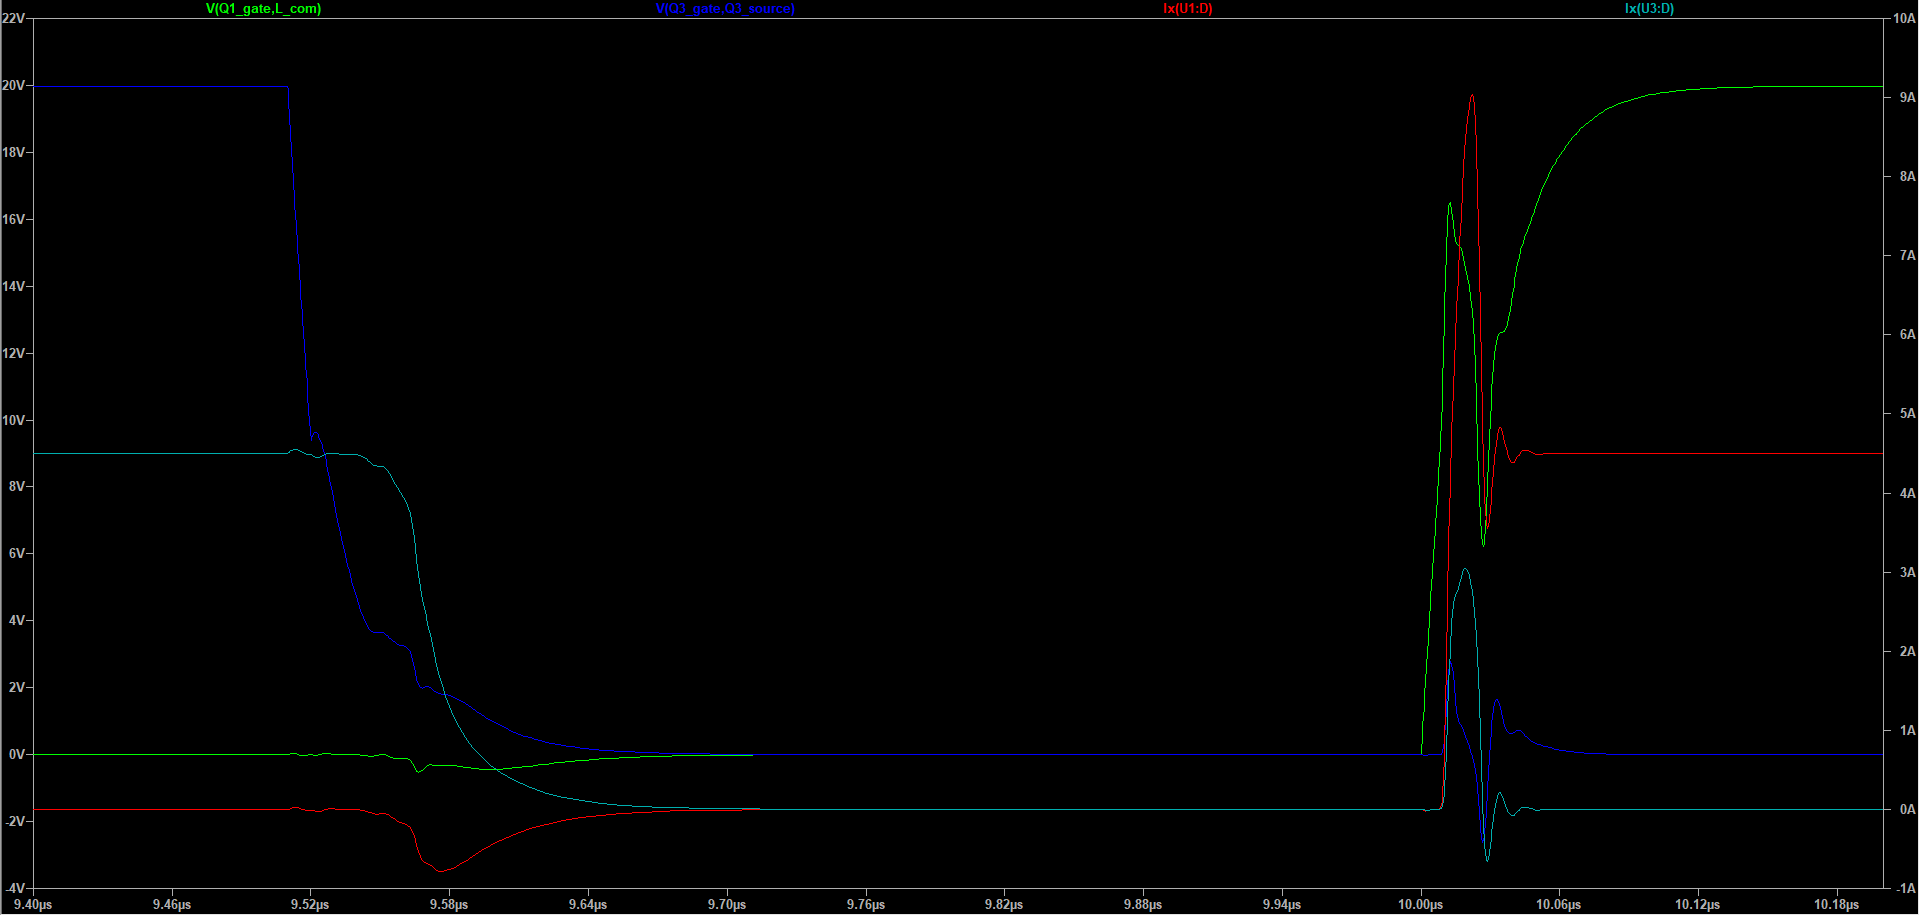
\includegraphics[width=\textwidth]{pictures/implementation/cap/cap_gates_3.PNG}
	\caption{Q3 turn off transient, gate voltages and drain currents}
	\label{fig:cap_gates_3}
\end{figure}

\begin{figure}[H]
	\centering
	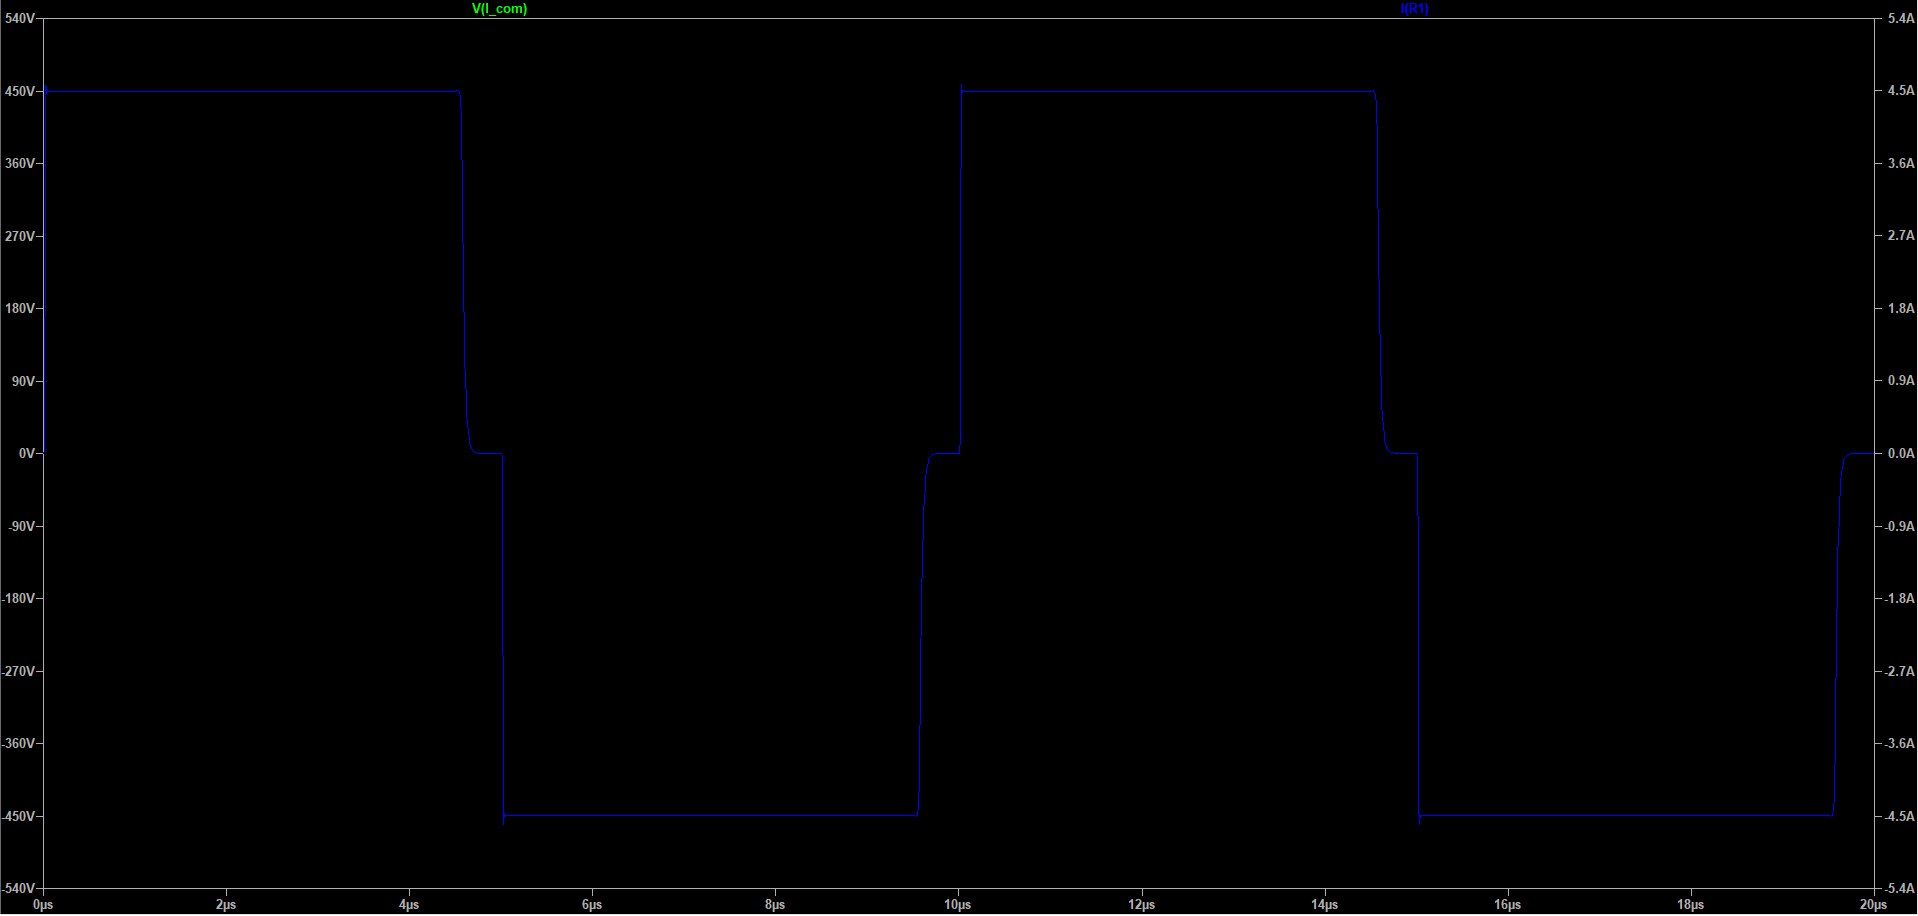
\includegraphics[width=\textwidth]{pictures/implementation/cap/cap_load.PNG}
	\caption{Voltage and current waveforms of the resistor overlap}
	\label{fig:cap_load}
\end{figure}

% Limitations, further possibilities
\input{sections/implementation/further.tex}

% Example
\subsection{Example: Extractions}
\label{sec:extraction}

The goal of this section is to provide a step-by-step description of the parasitic extraction process for future reference. Other students may find a tutorial of this kind helpful just as it is a good baseline for our upcoming work. \\

It was possible to extract parasitic inductance and resistance between various points within the nets. The following presents the step-by-step method of extracting the parasitic between two points, Q1 Drain and C11, that lies in one net, the DC+. Using a similar method, parasitic throughout different branches of the circuit were later extracted. The values are then added to the SPICE model for analyses.\\

\subsubsection{Setting up}

\begin{enumerate}
\item A schematic of one leg of a DC-DC converter was provided. It was studied to understand the scope of analysis. For the project, it was used as an inverter for the reasons laid out in Section \ref{sec:overview}.


\begin{figure} [H]
  \centering
  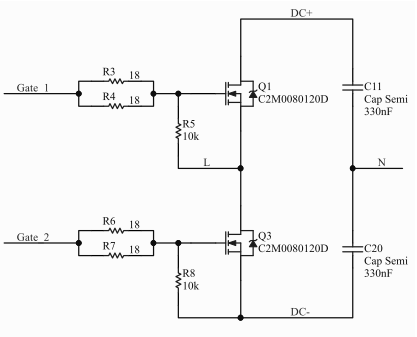
\includegraphics[width=\linewidth]{pictures/examples/main_schematic}
  \caption{Main Schematic of the circuit}
  \label{fig:main_schematic}
\end{figure}

\item A spice model was created based on the schematic which will be used to analyze the circuit once parasitic components from various branches of the circuit are extracted.

\begin{figure} [H]
  \centering
  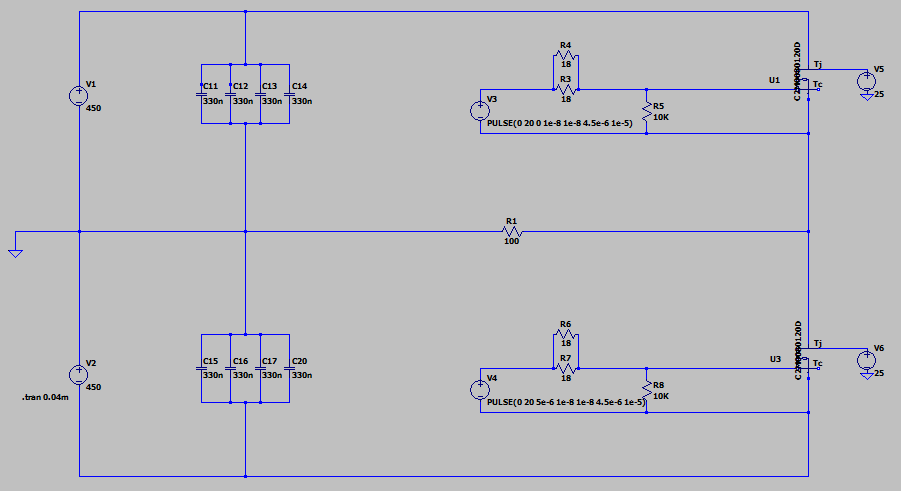
\includegraphics[width=\linewidth]{pictures/examples/spice.png}
  \caption{SPICE Model}
  \label{fig:main_spice}
\end{figure}

\item A 3D PCB Graphics layout was provided in PDF to identify the various components of the model. Analysis is not possible on this layout. It is provided only for component identification.

\begin{figure} [H]
  \centering
  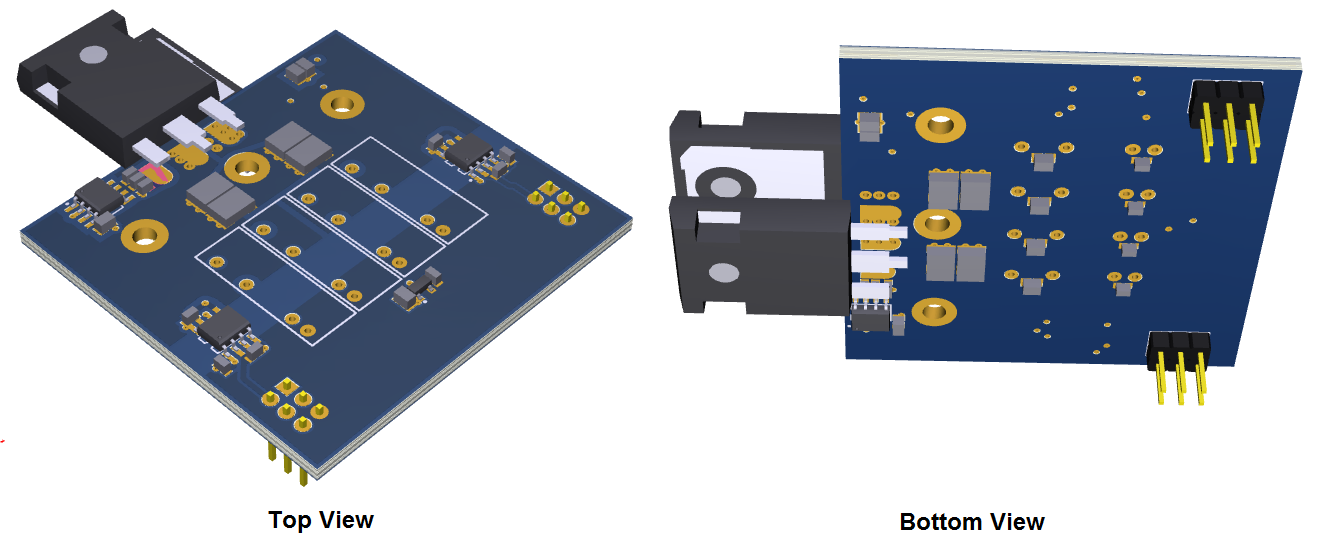
\includegraphics[width=\linewidth]{pictures/examples/PCB.png}
  \caption{3D PCB Layout in PDF}
  \label{fig:pcb}
\end{figure}

\item ODB++ files were provided which were imported to ANSYS SIwave to create the working 3D PCB Layout. Actual analysis is done on this layout.

\begin{figure} [H]
  \centering
  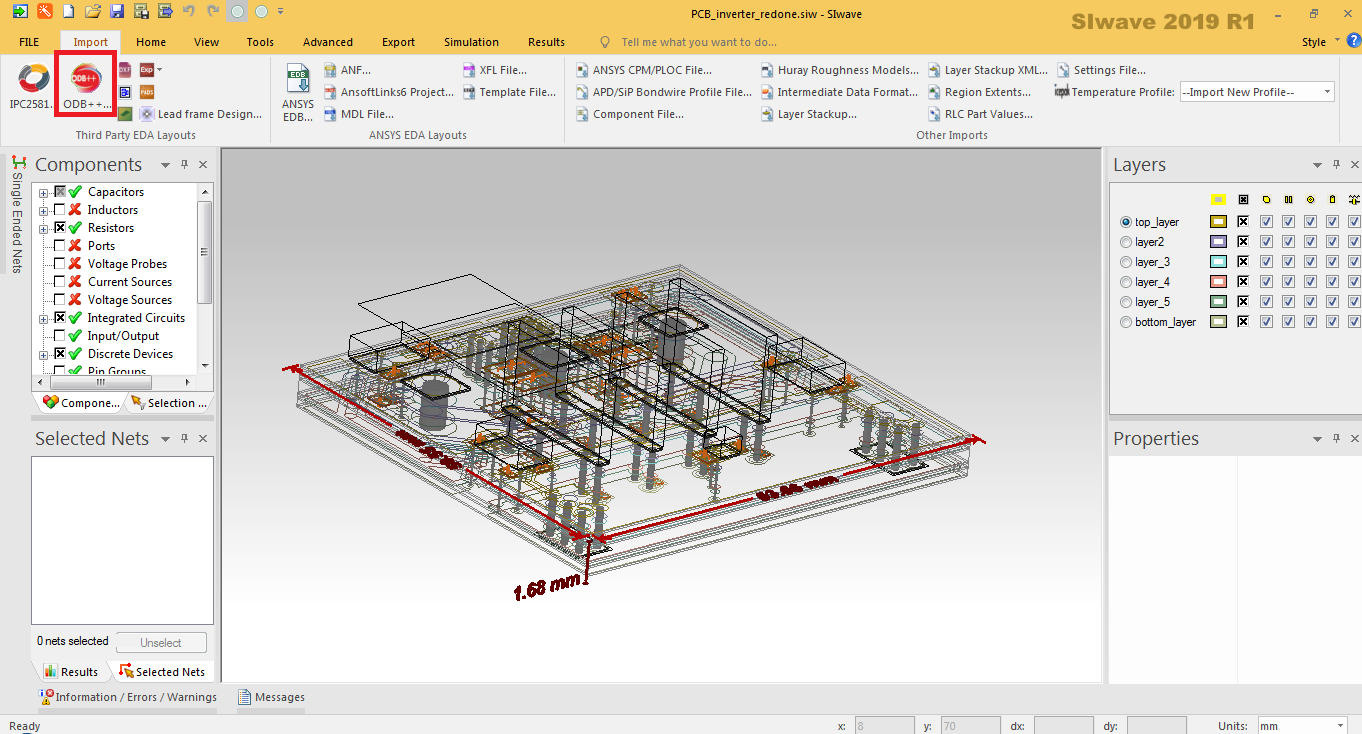
\includegraphics[width=\linewidth]{pictures/examples/siwave.png}
  \caption{ODB++ imported to create 3D PCB layout in ANSYS SIwave}
  \label{fig:siwave}
\end{figure}

\item The part of interest was cut from the 3D PCB layout and exported to Q3D extractor for extracting the values of the parasitic components.

\begin{figure} [H]
  \centering
  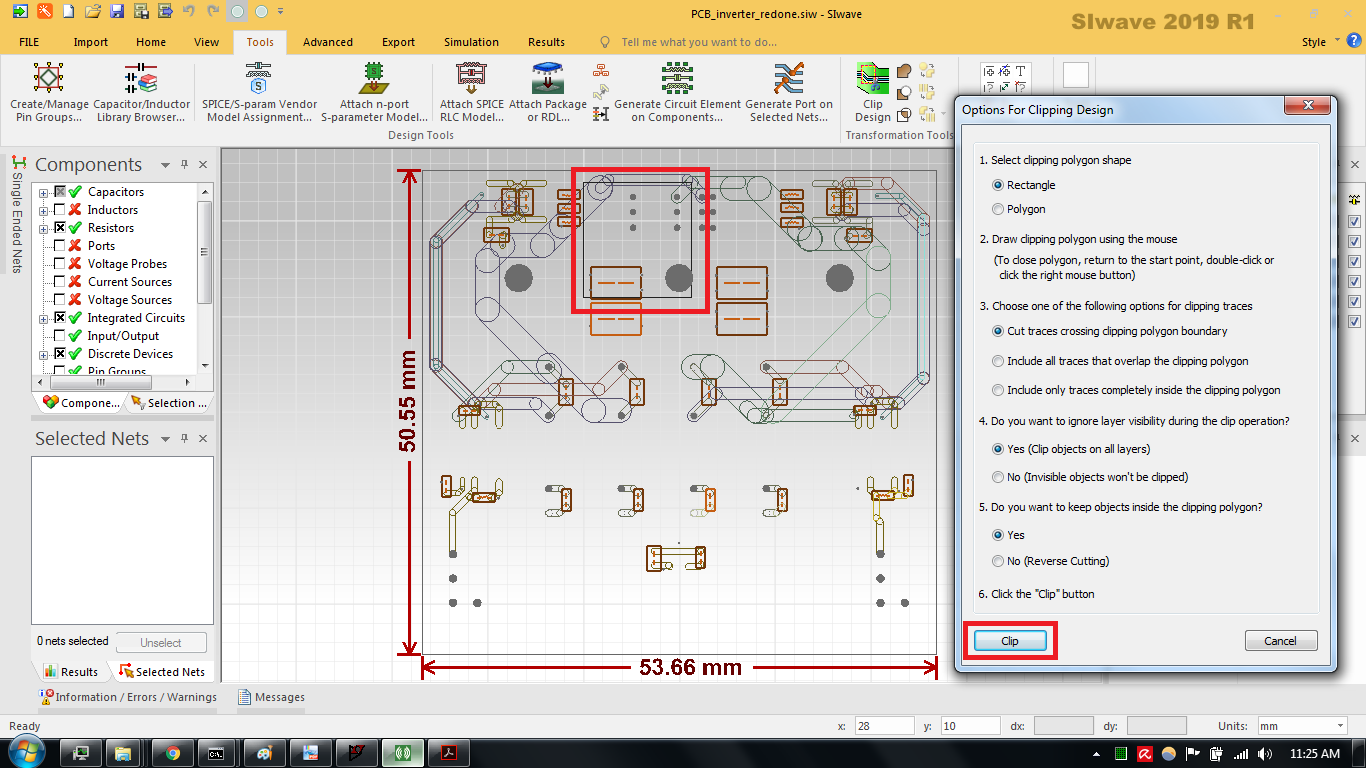
\includegraphics[width=\linewidth]{pictures/examples/siwave_clip2.png}
  \caption{The red box indicates the part of interest which will be cut and extracted to Q3D Extractor}
  \label{fig:siwave_cut}
\end{figure}

\end{enumerate}

\subsubsection{Step-by-step extraction process for parasitic inductance and resistance between Q1-Drain and C11 in the DC+ Net}

\begin{enumerate}
\item  First, we need to identify the two point in the schematic between which the parasitic is to be extracted. The points of interest must be in the same net. It is seen that the part of interest is the branch from Q1-Drain to C11 connected by the DC+ net.

\begin{figure} [H]
  \centering
  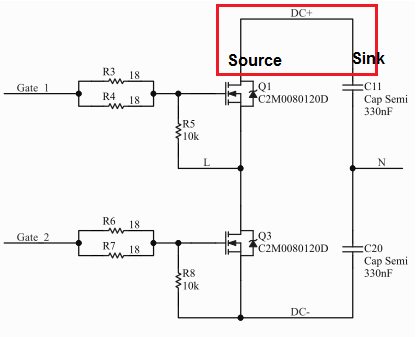
\includegraphics[width=\linewidth]{pictures/examples/Schematic1.png}
  \caption{The red box indicates the portion from where parasitic is extracted}
  \label{fig:schematic1}
\end{figure}

\item  The target is also marked in the corresponding SPICE model since the extracted parasitic components will be included in this particular branch.

\begin{figure} [H]
  \centering
  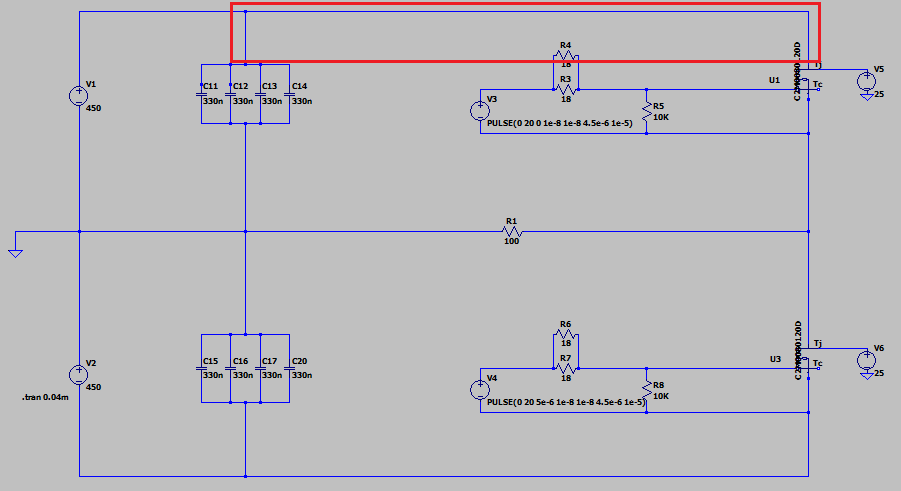
\includegraphics[width=\linewidth]{pictures/examples/spice1.png}
  \caption{The red box indicates the portion where the extracted parasitic is to be placed}
  \label{fig:spice1}
\end{figure}

\item Figure \ref{fig:PCB_cut1} depicts the section of the PDF PCB layout to be used for extraction. It shows the areas of Q1 drain and C11 on net DC+, while all other components are ignored. 

\begin{figure} [H]
  \centering
  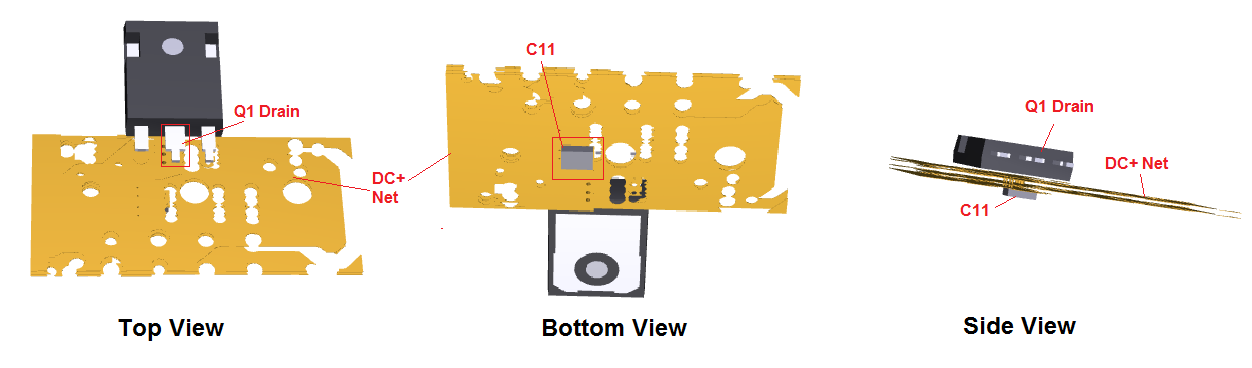
\includegraphics[width=\linewidth]{pictures/examples/PCB_cut_1.png}
  \caption{Portion of PCB that is of concern}
  \label{fig:PCB_cut1}
\end{figure}

\item Next, the PDF graphics layout is used to identify the part of interest within the net DC+ where the areas Q1-Drain and C11 are located in the ANSYS SIwave 3D PCB layout and that portion is clipped.

\begin{figure} [H]
  \centering
  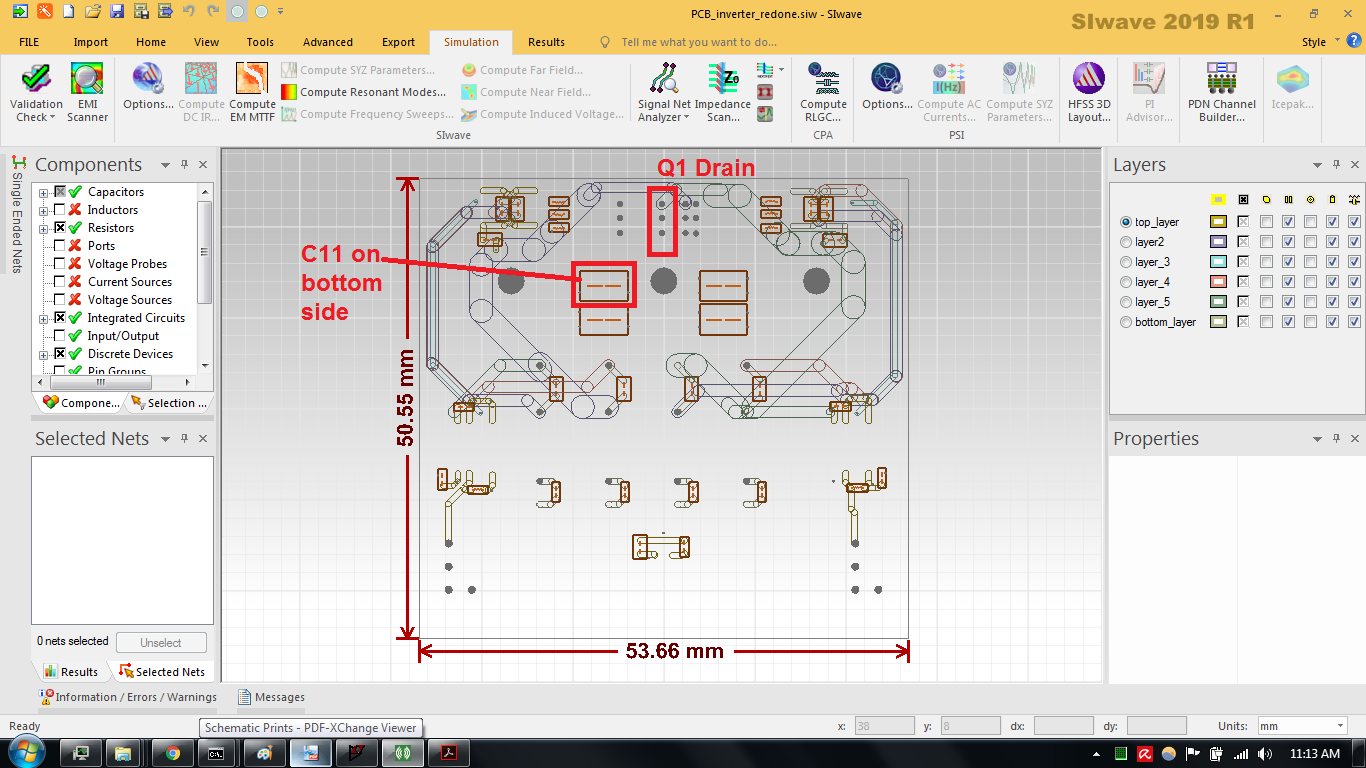
\includegraphics[width=\linewidth]{pictures/examples/siwave_td.png}
  \caption{Identifying Q1-Drain and C11 from top-down view}
  \label{fig:PCB_identify1}
\end{figure}

\begin{figure} [H]
  \centering
  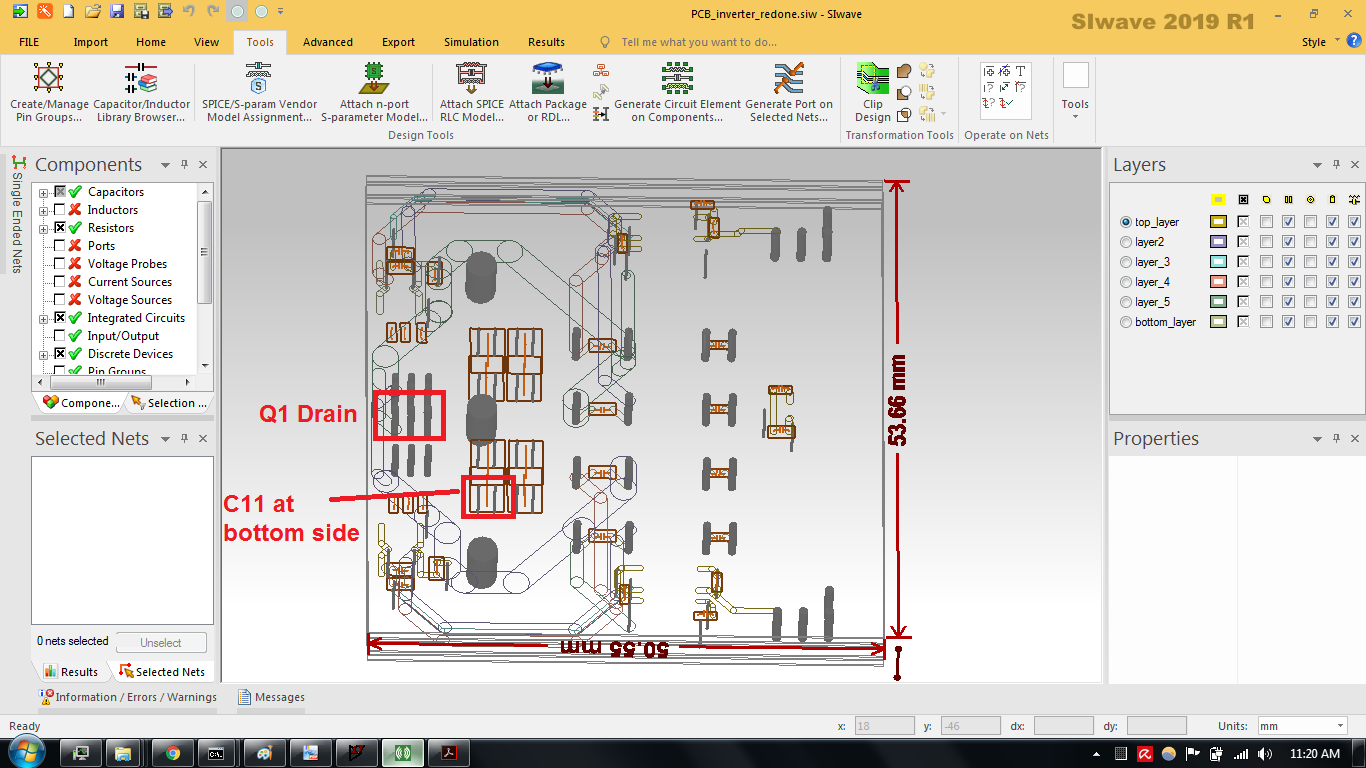
\includegraphics[width=\linewidth]{pictures/examples/siwave_ls.png}
  \caption{Identifying Q1-Drain and C11 from left side view}
  \label{fig:PCB_clip1}
\end{figure}

\begin{figure} [H]
  \centering
  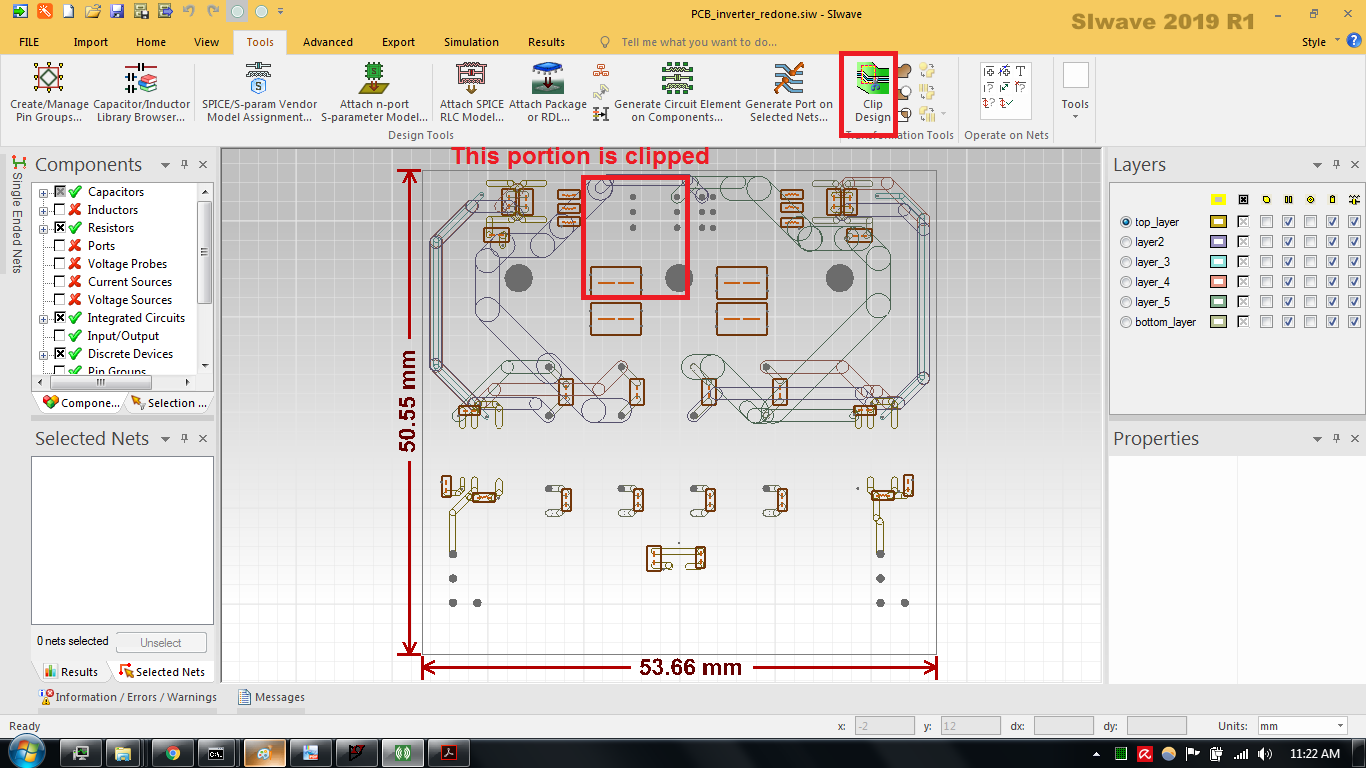
\includegraphics[width=\linewidth]{pictures/examples/siwave_clip1.png}
  \caption{Portion of PCB that is of concern containing all identified parts}
  \label{fig:PCB_clip1}
\end{figure}

\begin{figure} [H]
  \centering
  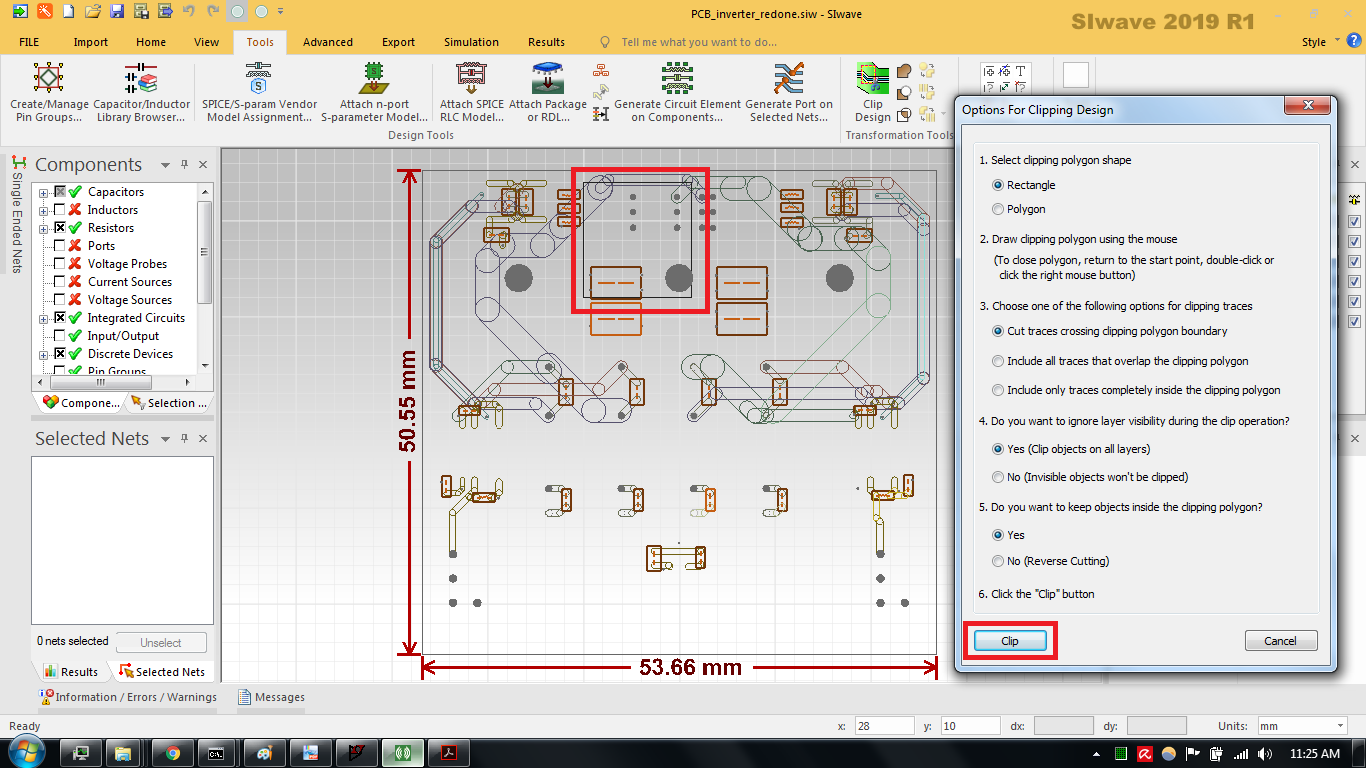
\includegraphics[width=\linewidth]{pictures/examples/siwave_clip2.png}
  \caption{Identified portion of PCB is clipped}
  \label{fig:PCB_clip2}
\end{figure}

\begin{figure} [H]
  \centering
  \includegraphics[width=\linewidth]{pictures/examples/siwave_clipped_td.png}
  \caption{Clipped part of the original PCB layout}
  \label{fig:PCB_clipped}
\end{figure}

\item The clipped portion is properly checked and verified to contain the part of interest. Repeat step 4 if clipping seems to have an error.

\begin{figure} [H]
  \centering
  \includegraphics[width=\linewidth]{pictures/examples/siwave_clipped_side.png}
  \caption{Verifying the clipped part of the original PCB layout}
  \label{fig:PCB_verified}
\end{figure}

\item The clipped portion is exported to ANSYS Q3D Extractor to extract the parasitic components.

\begin{figure} [H]
  \centering
  \includegraphics[width=\linewidth]{pictures/examples/siwave_export_q3d.png}
  \caption{Clipped PCB part is exported to ANSYS Q3D}
  \label{fig:siwave_q3d}
\end{figure}

\begin{figure} [H]
  \centering
  \includegraphics[width=\linewidth]{pictures/examples/Q1d_C11T_1.png}
  \caption{Top View of PCB Layout in Q3D}
  \label{fig:q3d1}
\end{figure}

\begin{figure} [H]
  \centering
  \includegraphics[width=\linewidth]{pictures/examples/Q1d_C11T_2.png}
  \caption{Bottom View of PCB Layout in Q3D}
  \label{fig:q3d2}
\end{figure}

\item In ANSYS Q3D, clipped PCB part containing the net DC+ is analyzed to recover the parasitic components\\

To find the parasitic components, we need to cover:
\begin{enumerate}
\item The area of the Q1-Drain and 
\item The area of the C11
\end{enumerate}
with a sheet on top of their individual located surfaces. The sheet has to be made of the same material as the face on which it is being created. In this case, it was copper.

\begin{figure} [H]
  \centering
  \includegraphics[width=\linewidth]{pictures/examples/Q1d_C11T_5.png}
  \caption{Q1-Drain area in the DC+ Net}
  \label{fig:Q1d}
\end{figure}

\begin{figure} [H]
  \centering
  \includegraphics[width=\linewidth]{pictures/examples/Q1d_C11T_6.png}
  \caption{C11 area in the DC+ Net}
  \label{fig:Q1d_C11t_sink}
\end{figure}

\item Assigning excitation, one of the two sheets is marked as source and the other as sink.

\begin{figure} [H]
  \centering
  \includegraphics[width=\linewidth]{pictures/examples/source.png}
  \caption{Assigning Source to Q1-Drain}
  \label{fig:source1}
\end{figure}

\begin{figure} [H]
  \centering
  \includegraphics[width=\linewidth]{pictures/examples/sink.png}
  \caption{Assigning Sink to C11}
  \label{fig:sink1}
\end{figure}

\begin{figure} [H]
  \centering
  \includegraphics[width=\linewidth]{pictures/examples/Q1d_C11T_7.png}
  \caption{Q1-Drain sheet assigned as Source}
  \label{fig:source2}
\end{figure}

\begin{figure} [H]
  \centering
  \includegraphics[width=\linewidth]{pictures/examples/Q1d_C11T_8.png}
  \caption{C11 sheet assigned as Sink}
  \label{fig:sink2}
\end{figure}

\item Next, 'Validation Check' is done prior to analysis to check for any errors with the design that might prevent the extraction process.

\begin{figure} [H]
  \centering
  \includegraphics[width=\linewidth]{pictures/examples/valid.png}
  \caption{'Validation Check' returns no error}
  \label{fig:valid}
\end{figure}

\item Since 'Validation Check' returned no error, after adding 'Solution Setup', the final step 'Analysis' is carried out to extract the parasitic components

\begin{figure} [H]
  \centering
  \includegraphics[width=\linewidth]{pictures/examples/solution.png}
  \caption{Add Solution Setup to configure the analysis requirements}
  \label{fig:solution}
\end{figure}

\begin{figure} [H]
  \centering
  \includegraphics[width=\linewidth]{pictures/examples/setup.png}
  \caption{Analysis is configured through 'Add Solution Setup'}
  \label{fig:setup}
\end{figure}

\begin{figure} [H]
  \centering
  \includegraphics[width=\linewidth]{pictures/examples/analysis.png}
  \caption{Finally 'Analyze' is done}
  \label{fig:setup}
\end{figure}

\begin{figure} [H]
  \centering
  \includegraphics[width=\linewidth]{pictures/examples/results.png}
  \caption{Solution showing the parasitic components}
  \label{fig:results}
\end{figure}

\item In the end, the extracted parasitic components are collected and added to the SPICE model. Parasitic components from other branches of the circuit are extracted using similar method and when all the branches are solved, analysis is done on the SPICE model to compare the ideal model (without the parasitic components) and the extracted model (with the parasitic components)

\begin{figure} [H]
  \centering
  \includegraphics[width=\linewidth]{pictures/examples/spice2.png}
  \caption{Parasitic inductance added to the SPICE model}
  \label{fig:results}
\end{figure}

\end{enumerate}

\subsubsection{Other examples of extracting parasitic inductance and resistance}
\label{sec:other_ind_res}

The images below gives two more examples showing how ANSYS was used to harvest the parasitic information between 2 branches of the circuit.

\subsubsection{Extraction between Q3-Source and C16 in the DC- Net}
\label{sec:extraction_q3s_c16}

In the schematic, this is the part from where the parasitic is extracted.

\begin{figure} [H]
  \centering
  \includegraphics[width=\linewidth]{pictures/examples/schematic2.png}
  \caption{The red box indicates the portion from where parasitic is extracted}
  \label{fig:schematic2}
\end{figure}

\begin{figure} [H]
  \centering
  \includegraphics[width=\linewidth]{pictures/examples/spice3.png}
  \caption{The red box indicates the portion where the extracted parasitic is to be placed}
  \label{fig:spice3}
\end{figure}

From the PCB layout, if we ignore all other parts except the Net and the areas from where the parasitic is extracted, the layout looks like the following

\begin{figure} [H]
  \centering
  \includegraphics[width=\linewidth]{pictures/examples/PCB_cut2.png}
  \caption{Portion of PCB that is of concern}
  \label{fig:PCB_cut2}
\end{figure}

In ANSYS Q3D, we analyze the PCB part to find the parasitic components

\begin{figure} [H]
  \centering
  \includegraphics[width=\linewidth]{pictures/examples/Q3S_C16_Source.png}
  \caption{Marking the Source position at Q3-Source in the DC- Net}
  \label{fig:Q3s_C16_source}
\end{figure}

\begin{figure} [H]
  \centering
  \includegraphics[width=\linewidth]{pictures/examples/Q3S_C16_Sink.png}
  \caption{Marking the Sink position at C16 in the DC- Net}
  \label{fig:Q3s_C16_sink}
\end{figure}

\begin{figure} [H]
  \centering
  \includegraphics[width=\linewidth]{pictures/examples/Q3S_C16_extractions.png}
  \caption{Extracted parasitic components}
  \label{fig:Q33_C16_extractions}
\end{figure}

\subsubsection{Extraction between C11 and C20 in the N Net}
\label{sec:extraction_c11_c20}

In the schematic, this is the part from where the parasitic is extracted

\begin{figure} [H]
  \centering
  \includegraphics[width=\linewidth]{pictures/examples/schematic3.png}
  \caption{The red box indicates the portion from where parasitic is extracted}
  \label{fig:schematic3}
\end{figure}

From the PCB layout, if we ignore all other parts except the Net and the areas from where the parasitic is extracted, the layout looks like the following.

\begin{figure} [H]
  \centering
  \includegraphics[width=\linewidth]{pictures/examples/PCB_cut_3.png}
  \caption{Portion of PCB that is of concern}
  \label{fig:PCB_cut3}
\end{figure}

\begin{figure} [H]
  \centering
  \includegraphics[width=\linewidth]{pictures/examples/spice4.png}
  \caption{The red box indicates the portion where the extracted parasitic is to be placed}
  \label{fig:spice4}
\end{figure}

In ANSYS Q3D, we analyze the PCB part to find the parasitic components.

\begin{figure} [H]
  \centering
  \includegraphics[width=\linewidth]{pictures/examples/c11_c20_source.png}
  \caption{Marking the Source position at C11 in the N Net}
  \label{fig:C11_C20_source}
\end{figure}

\begin{figure} [H]
  \centering
  \includegraphics[width=\linewidth]{pictures/examples/Q3S_C16_Sink.png}
  \caption{Marking the Sink position at C20 in the N Net}
  \label{fig:C11_C20_sink}
\end{figure}

\begin{figure} [H]
  \centering
  \includegraphics[width=\linewidth]{pictures/examples/Q3S_C16_extractions.png}
  \caption{Extracted parasitic components}
  \label{fig:C11_C20_extractions}
\end{figure}

\subsubsection{Step-by-step extraction process for parasitic capacitance between Q1-Gate and Q1-Drain}

The exact same procedure mentioned in Section 6.6.2 Step 1 - 6 is followed. From Step 7, extracting parasitic capacitance differs from how parasitic inductance and resistance is retrieved.

\begin{enumerate}

\item First, we need to target from the schematic:

\begin{figure} [H]
  \centering
  \includegraphics[width=\linewidth]{pictures/examples/Schematic5.png}
  \caption{The red box indicates the portion from where parasitic is extracted}
  \label{fig:schematic5}
\end{figure}

\item  The target is also marked in the corresponding SPICE model since the extracted parasitic components will be included between these particular branches.

\begin{figure} [H]
  \centering
  \includegraphics[width=\linewidth]{pictures/examples/spice5.png}
  \caption{The red box indicates the portion where the extracted parasitic is to be placed}
  \label{fig:spice5}
\end{figure}

\item From the PDF PCB layout, if all other components are ignored  except the Net DC+ (which contains the Q1-drain) and the net Q1-Gate from where the parasitic components are extracted, the layout looks like the following.

\begin{figure} [H]
  \centering
  \includegraphics[width=\linewidth]{pictures/examples/PCB_cut_4.png}
  \caption{Portion of PCB that is of concern}
  \label{fig:PCB_cut4}
\end{figure}

\item Next, the PDF graphics layout is used to identify the part of interest where both the nets DC+ (containing Q1-Drain) and Q1-gate overlaps. Then, the same area is located in the ANSYS SIwave 3D PCB layout and that portion is clipped.

\begin{figure} [H]
  \centering
  \includegraphics[width=\linewidth]{pictures/examples/siwave_td2.png}
  \caption{Identifying overlapped area of Q1-Gate and Q1-Drain from top-down view}
  \label{fig:PCB_identify2}
\end{figure}

\begin{figure} [H]
  \centering
  \includegraphics[width=\linewidth]{pictures/examples/siwave_clip3.png}
  \caption{Clipped Portion of PCB that is of concern containing the overlapped nets of Q1-Drain and Q1-Source}
  \label{fig:PCB_clip3}
\end{figure}

\item The clipped portion is properly checked and verified to contain the part of interest. Repeat step 4 if clipping seems to have an error.

\begin{figure} [H]
  \centering
  \includegraphics[width=\linewidth]{pictures/examples/siwave_verified.png}
  \caption{Verifying the clipped part of the original PCB layout}
  \label{fig:PCB_verified2}
\end{figure}

\item The clipped portion is exported to ANSYS Q3D Extractor to extract the parasitic components.

\begin{figure} [H]
  \centering
  \includegraphics[width=\linewidth]{pictures/examples/cap_q1_g_d}
  \caption{Clipped PCB part is exported to ANSYS Q3D}
  \label{fig:cap_q1_g_d}
\end{figure}

\item In ANSYS Q3D, the clipped PCB part where the Q1 gate and drain overlap is analyzed to recover the parasitic components.\\

To find the parasitic components, we need to:
\begin{enumerate}
\item Make one of them Signal - Here, Q1 gate is assigned Signal 
\item The one of then Ground - Here, Q1 drain (in the DC+ net) is assigned Ground 
\end{enumerate}

\begin{figure} [H]
  \centering
  \includegraphics[width=\linewidth]{pictures/examples/Q1d_verified2.png}
  \caption{Q1-Gate set as Signal and Q1-Drain set as Ground}
  \label{fig:PCB_verified3}
\end{figure}

\item Next, similar to Section 6.2.2. Step 9, 'Validation Check' is done prior to analysis to check for any error with the design that might prevent the extraction process

\item If, 'Validation Check' returned no error, similar to Section 6.2.2. Step 10, after adding 'Solution Setup', the final step, which is 'Analysis' is carried out to extract the parasitic components.

\begin{figure} [H]
  \centering
  \includegraphics[width=\linewidth]{pictures/examples/results2.png}
  \caption{Solution showing the parasitic components}
  \label{fig:results2}
\end{figure}

\item In the end, the extracted parasitic component is collected and added to the SPICE model. Parasitic capacitance from other areas where the nets overlap as shown in Section 6.5 (Q1 gate and source, Q1 drain and source, Q3 gate and drain, Q3 gate and source, Q3 drain and source) are extracted using similar method and when all are solved, analysis is done on the SPICE model to compare between the ideal model (without the parasitic components) and the extracted model (with the parasitic components).

\begin{figure} [H]
  \centering
  \includegraphics[width=\linewidth]{pictures/examples/spice6.png}
  \caption{Parasitic capacitance added to the spice model}
  \label{fig:results2}
\end{figure}

\end{enumerate}

Parasitic capacitance extracted between other nets are given in Section 6.5.

\newpage
% Discussion
\section{Discussion}
\label{sec:discussion}

The waveforms obtained in each stage of the modelling process look plausible. They exhibit minimal ringing at the switching events without causing false turn on - turn off cycles. \\

The factory-provided model of the MOSFET supports thermal simulations. This was not used, the junction temperature was fixed at 25 \textcelsius. This corresponds to the datasheet conditions. \\

Ideal, linear components were used to populate the schematic. They are supposed to be good models at the operating conditions. \\

Using the ANSYS suite is rather cumbersome. We are not sure that the process we have found for extracting parasitics is the right way or the easiest way. Input from someone more acquainted with the program would be welcome. \\

In order to confirm the pertinence of the model, laboratory measurements should be performed on the real circuit. If they show closely matching results, investigating a more tightly integrated circuit is the next step.

\newpage
% Conclusion
\section{Conclusion}
\label{sec:conclusion}

A model of a switching power pole was created in LTSpice. It was complemented by lumped inductances and capacitances extracted from critical parts of the PCB layout. Simulation results exhibit realistic-looking waveforms. The pertinence of the model has to be verified by lab measurements.

\newpage
% Abbreviation list
\section{Abbreviation list}
\label{sec:abbreviation_list}

% abcdefghijklmnopqrstuvwxyz
\begin{table}[H]
\centering
\begin{tabular}{|r|l|}
\hline
\textbf{Abbreviation} & \textbf{Meaning}                                        \\ \hline
FET          & Field-Effect Transistor                                          \\ \hline
LTSpice      & Implementation of SPICE by Linear Technology/Analog Devices      \\ \hline
MOSFET       & Metal-Oxide-Semiconductor Field-Effect Transistor                \\ \hline
PCB          & Printed Circuit Board                                            \\ \hline
PCBA         & Printed Circuit Board Assembly                                   \\ \hline
SPICE        & Simulation Program with Integrated Circuit Emphasis \\ \hline

\end{tabular}
\caption{Abbreviation list}\label{Abbreviationlist}
\label{tab:variable_ids}
\end{table}


\newpage
\listoffigures

\newpage
% References
\section{References}
\label{sec:references}
All links to websites was working on the day of the hand-in \textit{16-12-2019}.

%to use the Reference \cite{Name of the source},

\begin{thebibliography}{9}

\bibitem{Toshiba_app_note}
Parasitic Oscillation and Ringing of Power MOSFETs, \\
\url{https://toshiba.semicon-storage.com/info/docget.jsp?did=59456}

\bibitem{mosfet}
CREE C2M0080120D MOSFET datasheet, \\
\url{https://www.wolfspeed.com/media/downloads/167/C2M0080120D.pdf}

\bibitem{mosfet_2}
CREE C2M0080120D MOSFET product site, \\
\url{https://www.wolfspeed.com/c2m0080120d}

\end{thebibliography}






\end{document}
